\documentclass[11pt,a4paper]{report}

% ---------------------------------------------------------------------------
% Packages
% ---------------------------------------------------------------------------
\usepackage[T1]{fontenc}
\usepackage[utf8]{inputenc}
\usepackage{lmodern}
\usepackage[scaled=0.92]{helvet}
\usepackage{geometry}
\geometry{a4paper, top=2.7cm, bottom=2.6cm, left=2.7cm, right=2.7cm}
\usepackage{xcolor}
\usepackage{graphicx}
\usepackage{booktabs}
\usepackage{tabularx}
\usepackage{array}
\usepackage{multirow}
\usepackage{enumitem}
\usepackage{microtype}
\usepackage{amsmath,amssymb}
\usepackage{titlesec}
\usepackage{tocloft}
\usepackage{fancyhdr}
\usepackage[most]{tcolorbox}
\usepackage{subcaption}
\usepackage{listings}
\usepackage{tikz}
\usetikzlibrary{arrows.meta,positioning,shapes.geometric,fit,backgrounds}
\usepackage[colorlinks=true,linkcolor=FNavy,citecolor=FTeal,urlcolor=FTeal,
            bookmarks=true,pdftitle={Fabula: A Neurosymbolic Engine for AI-Generated Mystery Games},
            pdfauthor={Hafiz Muhammad Hassan, Hassan Nawaz, Muhammad Ibrahim}]{hyperref}

% ---------------------------------------------------------------------------
% Palette and typography
% ---------------------------------------------------------------------------
\definecolor{FNavy}{HTML}{0B1220}
\definecolor{FInk}{HTML}{1B2430}
\definecolor{FGold}{HTML}{D9A441}
\definecolor{FGoldLight}{HTML}{F2D28B}
\definecolor{FCream}{HTML}{F7F1E3}
\definecolor{FMuted}{HTML}{6B7A8F}
\definecolor{FTeal}{HTML}{1F7A8C}
\definecolor{FCrimson}{HTML}{B23A48}
\definecolor{FGreen}{HTML}{4E7A51}

\newcommand{\reportauthor}{Hafiz Muhammad Hassan \and Muhammad Ibrahim \and Shanzey Shahid}
\newcommand{\reportinstitution}{National University of Computer and Emerging Sciences (FAST-NUCES), Lahore}
\newcommand{\reportdate}{November 2026}

\titleformat{\chapter}[display]
  {\normalfont\sffamily\bfseries\color{FNavy}}
  {\filright\sffamily\large\color{FGold}CHAPTER \thechapter}
  {6pt}
  {\Huge}
  [\vspace{4pt}{\color{FGold}\titlerule[1.3pt]}]
\titlespacing*{\chapter}{0pt}{-18pt}{26pt}

\titleformat{\section}[hang]
  {\normalfont\sffamily\Large\bfseries\color{FNavy}}
  {\thesection}{0.7em}{}
\titlespacing*{\section}{0pt}{18pt}{7pt}

\titleformat{\subsection}[hang]
  {\normalfont\sffamily\large\bfseries\color{FInk}}
  {\thesubsection}{0.6em}{}
\titlespacing*{\subsection}{0pt}{13pt}{4pt}

\titleformat{\subsubsection}[hang]
  {\normalfont\sffamily\normalsize\bfseries\color{FTeal}}
  {\thesubsubsection}{0.5em}{}
\titlespacing*{\subsubsection}{0pt}{10pt}{3pt}

\setlist[itemize]{leftmargin=1.4em, itemsep=2pt, topsep=3pt, parsep=0pt}
\setlist[enumerate]{leftmargin=1.6em, itemsep=2pt, topsep=3pt, parsep=0pt}

% Page geometry refinements
\setlength{\headheight}{22pt}
\addtolength{\topmargin}{-7pt}

% Header and footer
\pagestyle{fancy}
\fancyhf{}
\fancyhead[L]{\footnotesize\sffamily\color{FMuted}FABULA \textperiodcentered{} FINAL PROJECT REPORT}
\fancyhead[R]{\footnotesize\sffamily\color{FMuted}\nouppercase{\leftmark}}
\fancyfoot[C]{\footnotesize\sffamily\color{FMuted}\thepage}
\renewcommand{\headrulewidth}{0.35pt}
\renewcommand{\headrule}{\hbox to\headwidth{\color{FGold}\leaders\hrule height \headrulewidth\hfill}}
\fancypagestyle{plain}{%
  \fancyhf{}%
  \fancyfoot[C]{\footnotesize\sffamily\color{FMuted}\thepage}%
  \renewcommand{\headrulewidth}{0pt}%
}

% TOC styling
\renewcommand{\cftchapfont}{\sffamily\bfseries\color{FNavy}}
\renewcommand{\cftchappagefont}{\sffamily\bfseries\color{FNavy}}
\renewcommand{\cftsecfont}{\sffamily}
\renewcommand{\cftsecpagefont}{\sffamily}
\setlength{\cftbeforechapskip}{7pt}

% Captions
\captionsetup{font=small, labelfont={bf,sf,color=FNavy}, textfont={small,sf}, skip=5pt}
\captionsetup[sub]{font=footnotesize, labelfont={bf,sf,color=FNavy}, textfont={footnotesize,sf}}

% Boxes
\newtcolorbox{keybox}[1][]{enhanced, breakable, colback=FGold!7, colframe=FGold!75!black,
  boxrule=0.7pt, arc=3pt, left=9pt, right=9pt, top=7pt, bottom=7pt,
  colbacktitle=FGold!85!black, coltitle=white, fonttitle=\sffamily\bfseries\small,
  title={#1}}
\newtcolorbox{quotebox}[1][]{enhanced, breakable, colback=FNavy, colframe=FNavy,
  coltext=FCream, boxrule=0pt, arc=3pt, left=12pt, right=12pt, top=10pt, bottom=10pt,
  fontupper=\small}
\newtcolorbox{warnbox}[1][]{enhanced, breakable, colback=FCrimson!6, colframe=FCrimson!80!black,
  boxrule=0.6pt, arc=2pt, left=9pt, right=9pt, top=6pt, bottom=6pt,
  colbacktitle=FCrimson!85!black, coltitle=white, fonttitle=\sffamily\bfseries\small,
  title={#1}}

% Listings
\lstdefinestyle{bundle}{
  basicstyle=\ttfamily\footnotesize\color{FInk},
  backgroundcolor=\color{FNavy!4},
  frame=single, framerule=0.4pt, rulecolor=\color{FNavy!25},
  breaklines=true, columns=fullflexible, keepspaces=true,
  showstringspaces=false, numbers=none,
  xleftmargin=8pt, xrightmargin=8pt, aboveskip=7pt, belowskip=7pt
}
\lstdefinestyle{dsl}{
  basicstyle=\ttfamily\footnotesize\color{FInk},
  backgroundcolor=\color{FGreen!6},
  frame=single, framerule=0.4pt, rulecolor=\color{FGreen!50!black},
  breaklines=true, columns=fullflexible, keepspaces=true,
  showstringspaces=false, numbers=left, numberstyle=\tiny\color{FMuted},
  xleftmargin=18pt, xrightmargin=8pt, aboveskip=7pt, belowskip=7pt
}
\renewcommand{\lstlistingname}{Listing}

% Utility
\newcommand{\code}[1]{\texttt{\small #1}}
\newcommand{\good}[1]{\textcolor{FGreen}{\textbf{#1}}}
\newcommand{\bad}[1]{\textcolor{FCrimson}{\textbf{#1}}}
\setlength{\parskip}{2pt}
\setlength{\parindent}{0pt}
\widowpenalty=10000
\clubpenalty=10000

% ---------------------------------------------------------------------------
\begin{document}

% ===========================================================================
% COVER
% ===========================================================================
\begin{titlepage}
\thispagestyle{empty}
\hypersetup{pageanchor=false}
\begin{tikzpicture}[remember picture,overlay]
  % night sky
  \fill[FNavy] (current page.south west) rectangle (current page.north east);
  % stars
  \foreach \x/\y/\r in {
    1.2/27.6/1.0, 2.8/24.1/0.7, 4.4/28.4/0.6, 5.9/26.2/1.1, 7.4/28.8/0.5,
    8.6/23.4/0.8, 10.1/27.0/0.6, 11.8/25.1/1.0, 13.2/28.1/0.7, 14.6/23.9/0.5,
    16.1/26.8/0.9, 17.9/28.6/0.6, 19.2/24.8/0.7, 2.1/21.3/0.5, 3.7/19.6/0.9,
    6.3/21.9/0.6, 8.9/20.2/0.7, 11.1/22.4/0.5, 13.8/20.8/0.9, 15.9/22.9/0.6,
    18.3/21.1/0.5, 1.5/16.8/0.6, 4.9/17.9/0.5, 7.8/16.3/0.8, 10.4/18.4/0.5,
    12.9/17.2/0.6, 15.1/18.9/0.8, 17.4/16.5/0.5, 19.6/18.1/0.6, 2.7/13.1/0.5,
    5.4/14.2/0.6, 9.7/13.8/0.5, 12.2/14.9/0.6, 14.4/13.2/0.5, 16.8/14.6/0.6,
    18.9/12.8/0.5, 3.9/10.4/0.5, 7.1/11.2/0.5, 11.6/10.8/0.5, 15.4/11.6/0.5
  } {
    \fill[white!85!FGold, opacity=0.65]
      ([xshift=\x cm,yshift=\y cm]current page.south west) circle (\r pt);
  }
  % moon
  \fill[FGoldLight!70, opacity=0.22]
    ([xshift=16.9cm,yshift=23.7cm]current page.south west) circle (1.55cm);
  \fill[FGoldLight!85, opacity=0.90]
    ([xshift=16.9cm,yshift=23.7cm]current page.south west) circle (1.02cm);
  \fill[FNavy!12, opacity=0.55]
    ([xshift=16.55cm,yshift=24.02cm]current page.south west) circle (0.19cm);
  \fill[FNavy!10, opacity=0.45]
    ([xshift=17.22cm,yshift=23.36cm]current page.south west) circle (0.13cm);
  % gold frame
  \draw[FGold, line width=1.1pt]
    ([xshift=1.15cm,yshift=-1.15cm]current page.north west)
    rectangle ([xshift=-1.15cm,yshift=1.15cm]current page.south east);
  \draw[FGold, line width=0.4pt]
    ([xshift=1.35cm,yshift=-1.35cm]current page.north west)
    rectangle ([xshift=-1.35cm,yshift=1.35cm]current page.south east);
\end{tikzpicture}

\vspace*{1.1cm}
\begin{center}
  {\sffamily\small\color{FGold}\bfseries FINAL PROJECT REPORT}\\[1.5cm]
  {\sffamily\bfseries\fontsize{62}{66}\selectfont\color{FCream} FABULA}\\[0.55cm]
  {\sffamily\large\color{FCream!92} A Neurosymbolic Engine for}\\[2pt]
  {\sffamily\large\color{FCream!92} AI-Generated Mystery Games}\\[0.9cm]
  {\itshape\color{FGoldLight} Question the town. Catch the lie.}\\[1.5cm]
  {\color{FGold}\rule{10cm}{0.5pt}}\\[1.1cm]
  {\sffamily\small\color{FCream!75}
    \textsc{The Body} \;---\; deterministic clocks, schedules, perception, proof\\[3pt]
    \textsc{The Voice} \;---\; language-model characters behind a spoiler firewall}\\[2.6cm]
\end{center}

\vfill
\begin{center}
  {\sffamily\small\color{FCream!90}\bfseries
    HAFIZ MUHAMMAD HASSAN \quad\textperiodcentered\quad 24L-2610\\[2pt]
    MUHAMMAD IBRAHIM \quad\textperiodcentered\quad 24L-2602\\[2pt]
    SHANZEY SHAHID \quad\textperiodcentered\quad 22L-7451}\\[0.85cm]
  {\sffamily\footnotesize\color{FCream!70}
    National University of Computer and Emerging Sciences\\ (FAST-NUCES), Lahore}\\[0.45cm]
  {\sffamily\footnotesize\color{FGold}\reportdate}
\end{center}
\vspace*{0.9cm}
\end{titlepage}
\hypersetup{pageanchor=true}

% ===========================================================================
% FRONT MATTER
% ===========================================================================
\pagenumbering{roman}
\clearpage
\phantomsection
\addcontentsline{toc}{chapter}{Abstract}
\chapter*{Abstract}
\markboth{Abstract}{Abstract}

Fabula is a single-player mystery game in which every case is written before the player arrives. A fine-tuned language model produces a story intent; a deterministic compiler turns that intent into a validated game world; and a headless simulation engine runs a ten-minute investigation in a small town of five or six suspects. The player questions residents, examines locations, and finally accuses one suspect of the crime, naming the method and the motive.

This report describes the design, implementation, and evaluation of the two-tier neurosymbolic pipeline behind the game. The \emph{fast route} uses a QLoRA-tuned Llama-3.2-1B-Instruct model that emits a compact blueprint DSL of roughly 150 tokens; a pure-Python compiler expands it into the complete bundle---locations, cast, timeline, clues, and per-NPC memories---and proves candidate-elimination solvability before anything is published. A second, legacy route fine-tunes Qwen2.5-3B-Instruct to serialise the same contract stage by stage as JSON. During play, no language model runs locally: NPC movement and perception are deterministic, and conversation is delegated to live providers behind a strict per-NPC knowledge boundary, with a deterministic scripted fallback when no API key is available.

Across 44 measured generation runs the fast route was schema-valid and solvability-proved in 44/44 cases, averaged 9.03\,s end-to-end warm (31.0 tokens/s, 1.48\,GB peak RSS) on a consumer laptop CPU, and produced 31 distinct cases from 31 seeds. The staged 3B route averaged 657.7\,s (5.27 tokens/s, 3.55\,GB) over two valid runs and failed validation once---a $72.8\times$ end-to-end gap that motivates the blueprint design. A small qualitative rubric over four generated cases shows strong mystery coherence (4.25/5) and knowledge isolation (4.0/5), while identifying clue specificity and surface prose as the main quality gaps. The report closes with limitations and a concrete plan for closing those gaps.

\vspace{0.9cm}
\begin{keybox}[Contributions at a glance]
\begin{itemize}
  \item A \textbf{compact blueprint DSL} and symbolic compiler that move JSON syntax and bookkeeping out of the neural model, cutting generation from minutes to seconds without sacrificing schema validity.
  \item A \textbf{machine-enforced knowledge boundary} for NPC dialogue: the engine-only truth file never enters a prompt, and per-NPC isolation is verified by tests rather than prompt wording.
  \item A \textbf{reproducible evaluation harness} that records hardware, model hashes, per-stage timings, token counts, validation outcomes, solvability proofs, and repeatability across 44 runs.
  \item An end-to-end, \textbf{playable artefact}: 16 curated cases, a Pygame client, CLI generation, and a live-API/scripted conversation layer.
\end{itemize}
\end{keybox}

\tableofcontents
\clearpage
\phantomsection
\addcontentsline{toc}{chapter}{List of Figures}
\markboth{\listfigurename}{\listfigurename}
\listoffigures
\clearpage
\phantomsection
\addcontentsline{toc}{chapter}{List of Tables}
\markboth{\listtablename}{\listtablename}
\listoftables
\clearpage

% ===========================================================================
\pagenumbering{arabic}
\setcounter{page}{1}

\chapter{Introduction}
\label{ch:intro}

\section{The Game}
Fabula is a small, replayable detective game. The player arrives in a town of five or six residents, has ten minutes of in-game time, and must answer three questions: who committed the crime, how they did it, and why. The town contains four connected locations---a library, a market, a park, and a residence in the reference bundle---and four to six clues, some found by searching a place and others revealed by a resident during conversation. Every case is self-contained: one culprit, one authored cover story, and an evidence chain that should let an attentive player eliminate every innocent suspect.

What makes the game unusual is where the case comes from. It is generated on the player's machine before play begins, and it is compiled rather than merely prompted. The language model contributes premise, cast, motive, and the shape of the conspiracy; a deterministic compiler contributes the world graph, schedules, per-NPC memory files, accusation options, and a machine-checked solvability proof. The generated bundle is then played by an engine that has no neural component of its own. Language models return only for conversation---and even then they are optional.

\begin{figure}[htbp]
  \centering
  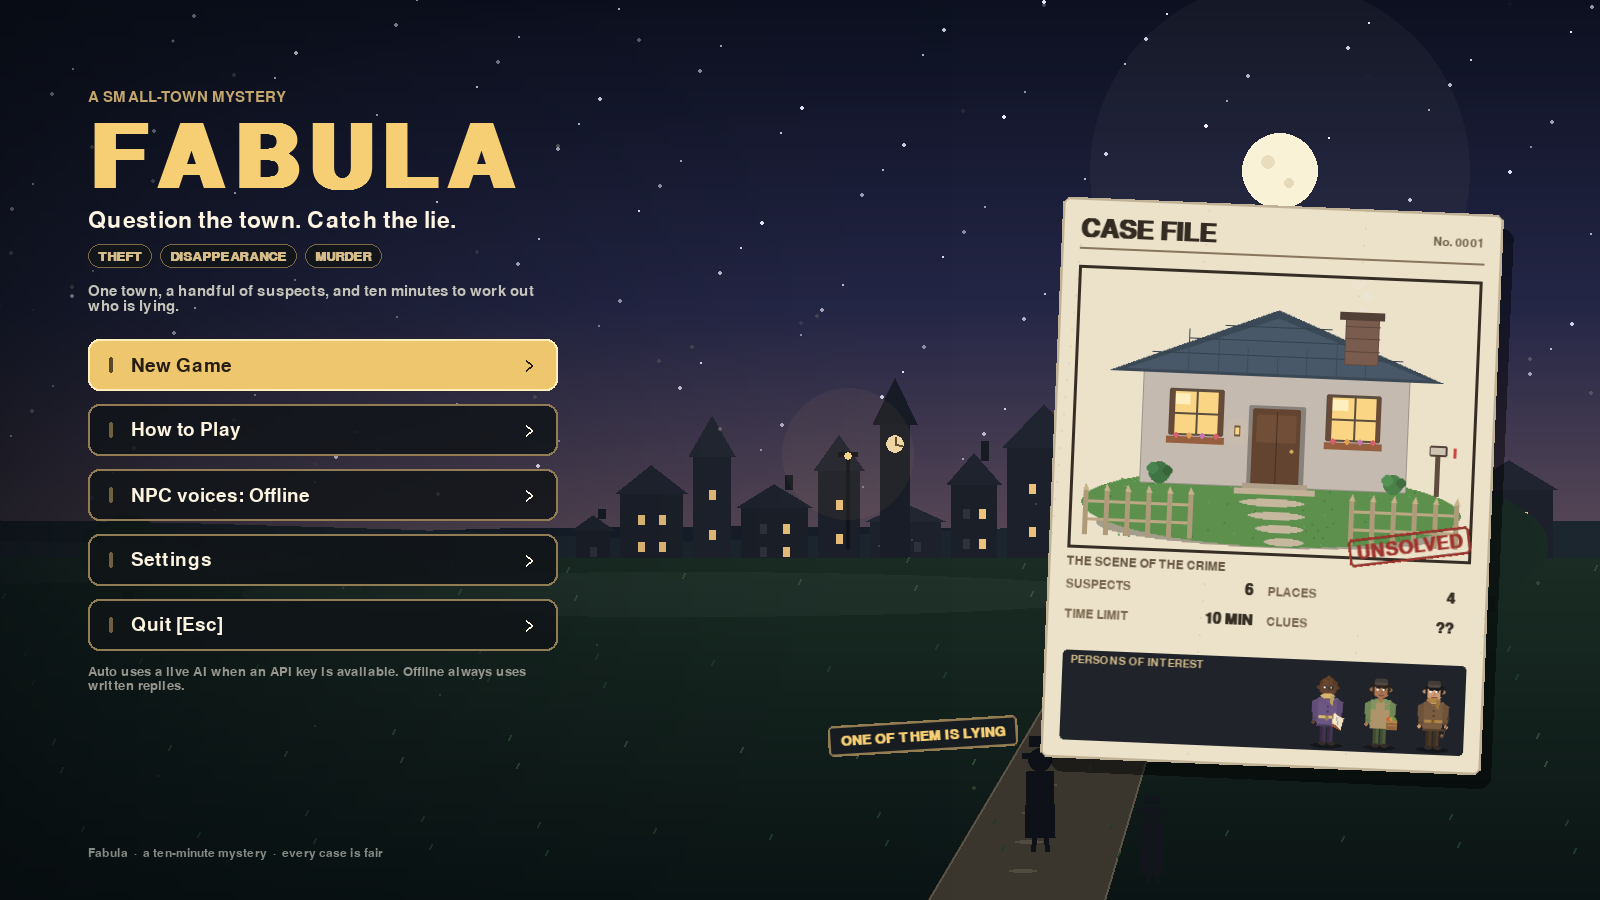
\includegraphics[width=0.92\textwidth]{figures/start_menu.png}
  \caption{The start menu. Case generation, ready-case selection, voice mode, and the how-to-play guide are reachable before a session begins.}
  \label{fig:menu}
\end{figure}

\begin{figure}[htbp]
  \centering
  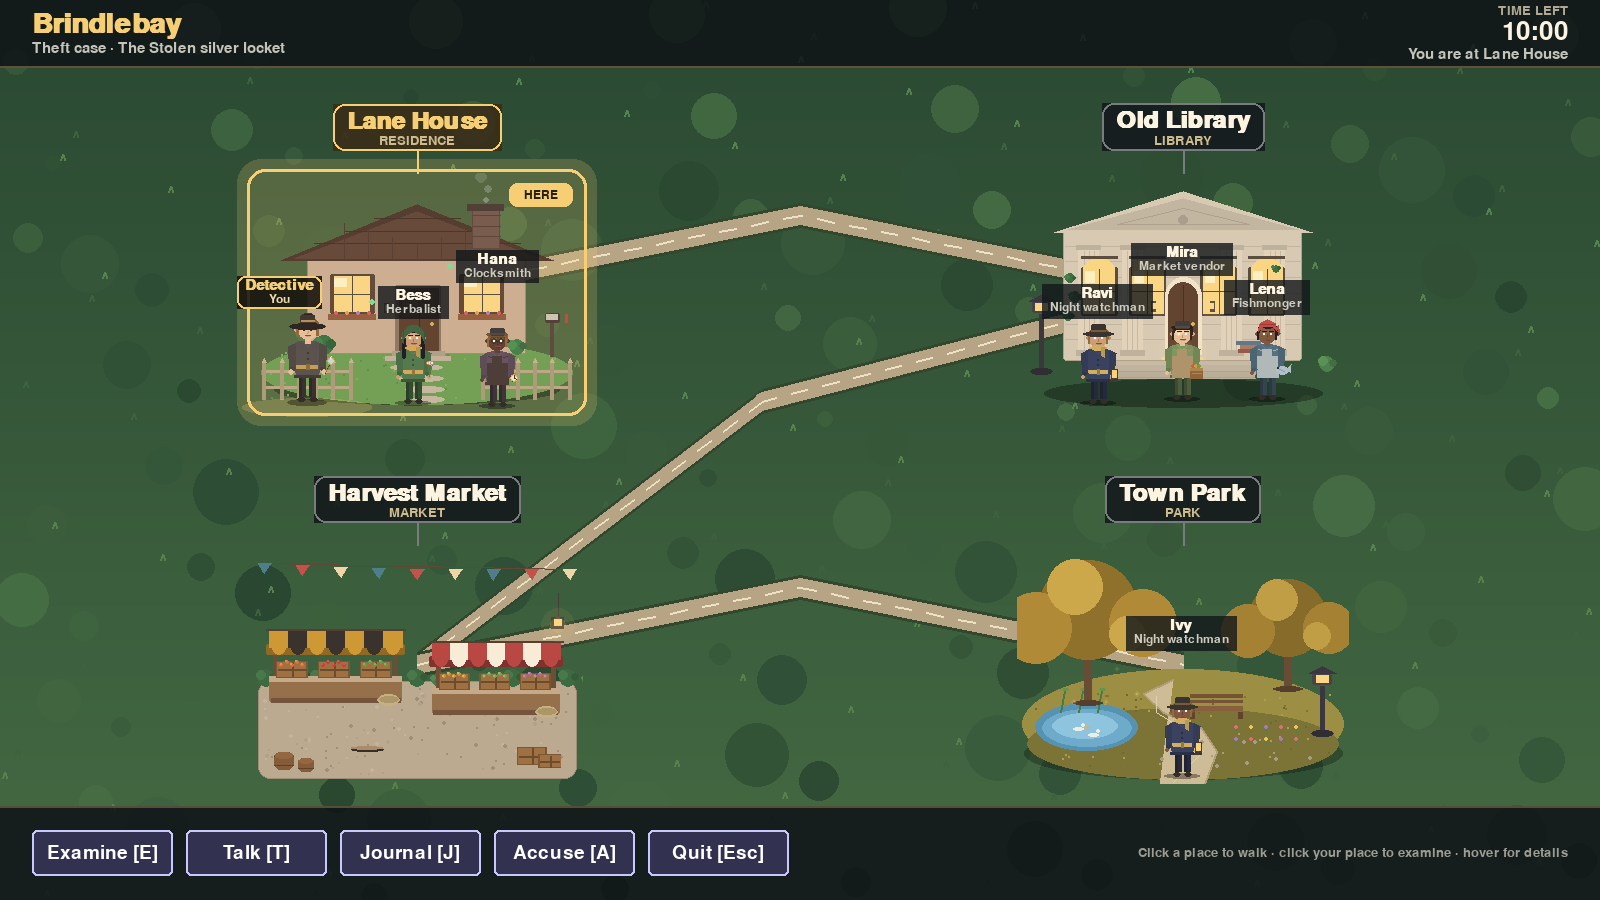
\includegraphics[width=0.92\textwidth]{figures/map.png}
  \caption{The town map. The detective (left) stands at the player's current location; NPCs are drawn where their schedules place them. The HUD shows the case title and the ten-minute countdown.}
  \label{fig:map}
\end{figure}

\section{Motivation}
Mystery fiction is an attractive target for generative play because its structure is simultaneously creative and formal. A good mystery needs an imaginative premise and believable motives, but it also needs a conspiracy that closes: a culprit, an opportunity, a method, a cover story, and clues whose implications eliminate the innocent. Language models are excellent at the first half and unreliable at the second. Asked for a complete case as JSON, a small model will happily invent a compelling town and then contradict the crime scene, omit the culprit's motive, or emit a clue that points at nobody.

There is a second, more practical motivation. A ten-minute game cannot spend ten minutes generating its content. Our first staged pipeline generated a case as nine sequential JSON stages and took tens of minutes on a laptop CPU: the model was being used as a database serialiser, paying the full cost of generating braces, keys, and repeated boilerplate. The blueprint route exists because that cost is avoidable. The model should write the \emph{story}; the engine should write the \emph{data}.

\section{Problem Statement}
The project addresses four coupled problems.

\begin{enumerate}
  \item \textbf{Latency.} A playable case must be generated on commodity hardware in well under a minute. The design ceiling is 15 seconds; the target is under seven.
  \item \textbf{Validity.} The generated world must satisfy a frozen schema, and every cross-file invariant---connected locations, scheduled NPCs, clue reachability, accusation options---must hold before the player sees it.
  \item \textbf{Solvability.} The evidence must be sufficient to identify exactly one culprit. A case that is merely schema-valid can still be unfair.
  \item \textbf{Knowledge isolation.} NPC dialogue must never leak the engine-only truth or another character's secrets. This has to be an architectural guarantee, not a request in a prompt.
\end{enumerate}

The project deliberately excludes several attractive but out-of-scope ideas: a runtime local chat model, generated art, a general planner, and machine-learned action selection. The game is small on purpose. The research question is not ``can an LLM run a town?'' but ``what is the smallest reliable division of labour between a neural writer and a symbolic engine that still produces a playable mystery?''

\section{Contributions}
\begin{itemize}
  \item \textbf{Neural sketch, symbolic completion.} We introduce a compact blueprint DSL (roughly 145--160 tokens) and a 823-line compiler that expands it into a complete, validated bundle while preserving the model's semantic choices. The compiler fills only structural gaps and never reassigns the culprit.
  \item \textbf{Proof before publication.} Every case passes a candidate-elimination check: exactly the culprit may own a clue-reachable secret \texttt{did} fact, and every innocent must have a clue-backed alibi. Bundles are published atomically only after schema and solvability checks pass.
  \item \textbf{A spoiler firewall enforced by construction.} The play-phase prompt assembler reads only the speaking NPC's identity, memory, and chat history. The truth file is not merely omitted from a template; it is unreachable from the conversation service, and automated tests assert the boundary.
  \item \textbf{An evidence-backed comparison.} We fine-tune, quantise, and measure both routes on the same machine, report validity and solvability separately from latency, and publish the raw run records. The fast route is 72.8 times faster end-to-end and uses 2.4 times less memory at equal validity.
\end{itemize}

\section{Report Organisation}
Chapter~\ref{ch:related} situates the work in generative agents, neurosymbolic AI, and fair-play mystery design. Chapter~\ref{ch:architecture} gives the two-phase architecture and the bundle contract. Chapter~\ref{ch:generation} details both generation routes and the solvability proof. Chapter~\ref{ch:data} covers the synthetic dataset, teacher expansion, distillation, and QLoRA training. Chapter~\ref{ch:play} describes the deterministic engine, the spoiler firewall, the conversation layer, and the interface. Chapter~\ref{ch:eval} reports the evaluation. Chapter~\ref{ch:discussion} discusses trade-offs, limitations, and future work, and Chapter~\ref{ch:conclusion} concludes.

\chapter{Background and Related Work}
\label{ch:related}

\section{Generative Agents and LLM Game AI}
The idea of language models as game characters gained prominence with \emph{Generative Agents} \cite{park2023generative}, where memory streams, reflection, and planning produced believable social behaviour in a small simulated town. ReAct \cite{yao2023react} interleaved reasoning and acting, and Voyager \cite{wang2023voyager} demonstrated open-ended skill acquisition in Minecraft. Earlier work on quest generation \cite{ammanabrolu2020quest} already showed that neural generation and symbolic game state can be combined, and that pure text generation struggles with the constraints a game engine requires.

Fabula borrows the ``town of agents'' framing but inverts the usual priority. The agents are not the product; the case is. NPC behaviour must be predictable enough to support deduction, so the simulation is classical and the language model is confined to speech. This is closer to a content pipeline with a conversational interface than to an autonomous agent society.

\section{Neurosymbolic AI}
Neurosymbolic systems combine learned perception or generation with symbolic reasoning and verification \cite{garcez2023neurosymbolic,kautz2022third}. The pattern is attractive precisely where LLMs are weakest: arithmetic, consistency, and constraints. Constrained decoding \cite{willard2023guided} is one lightweight form of the idea, forcing a model's output to remain inside a grammar. Fabula uses constrained decoding on the staged route, but its main architectural bet is stronger: \emph{do not ask the model to emit the data structure at all}. Ask it for a dense, low-syntax sketch, and let a compiler do the serialisation.

This division has a useful failure mode. If the model omits a structural requirement, the compiler can supply it deterministically from the model's own cast and timeline. If the model contradicts itself, the compiler can detect the contradiction during validation. The model remains the author of the mystery; it is no longer the author of its file format.

\section{Fair-Play Mystery Design}
Classical detective fiction codified fairness: the culprit must be present early, the clues must be available to the reader, and the solution must not depend on withheld supernatural knowledge \cite{knox1929decalogue,vandine1928rules}. Fabula operationalises a narrow, machine-checkable version of fairness. A clue's \texttt{implies} list names the facts it supports; the compiler computes which NPCs own clue-reachable facts; and the candidate set must collapse to exactly one culprit. Every innocent must also be clearable by a clue-backed alibi. This is not a literary theory of fairness, but it is a necessary condition, and it catches the most common generation failure: a vivid case with no deductive path to its own solution.

\section{Efficient Adaptation and Edge Inference}
QLoRA \cite{dettmers2023qlora} made it practical to fine-tune multi-billion-parameter models on a single consumer GPU, and LoRA \cite{hu2022lora} keeps the adapters small. We use Unsloth \cite{unsloth} for memory-efficient training on Kaggle Tesla T4s, then export to GGUF and run with \texttt{llama.cpp} \cite{llamacpp} on CPU. The student models are Llama-3.2-1B-Instruct \cite{llama3herd} and Qwen2.5-3B-Instruct \cite{qwen2025}; the choice is deliberate. A 1B model at four-bit precision is small enough to load in about a second and fast enough to generate a sketch in seconds, while a 3B model has more room for staged JSON but pays for it in memory bandwidth.

\section{Positioning}
Existing work tends to evaluate generated game content by human preference or by downstream task success. Fabula's evaluation separates three questions that are often conflated: \emph{is the artefact valid}, \emph{is it solvable}, and \emph{is it fast enough to play}. Narrative quality is assessed separately, with a small rubric, and reported as a qualitative case study rather than as a benchmark win. The result is a clearer picture of what the architecture buys and what it costs.

\chapter{System Architecture}
\label{ch:architecture}

\section{Two Phases}
Fabula has a hard boundary between \emph{generation} and \emph{play}. Generation happens before the player enters the town. It is allowed to be slow, expensive, and iterative; it must produce an immutable bundle on disk. Play begins when that bundle is loaded. It must be deterministic, responsive, and independent of any model file.

This split is the most important design decision in the project. It means that the expensive, failure-prone neural component can be tested, retried, versioned, and replaced without touching the runtime. It also means that a generated case is a first-class artefact: the same bundle can be played offline, archived, shared, or used as evaluation data.

\begin{figure}[htbp]
  \centering
  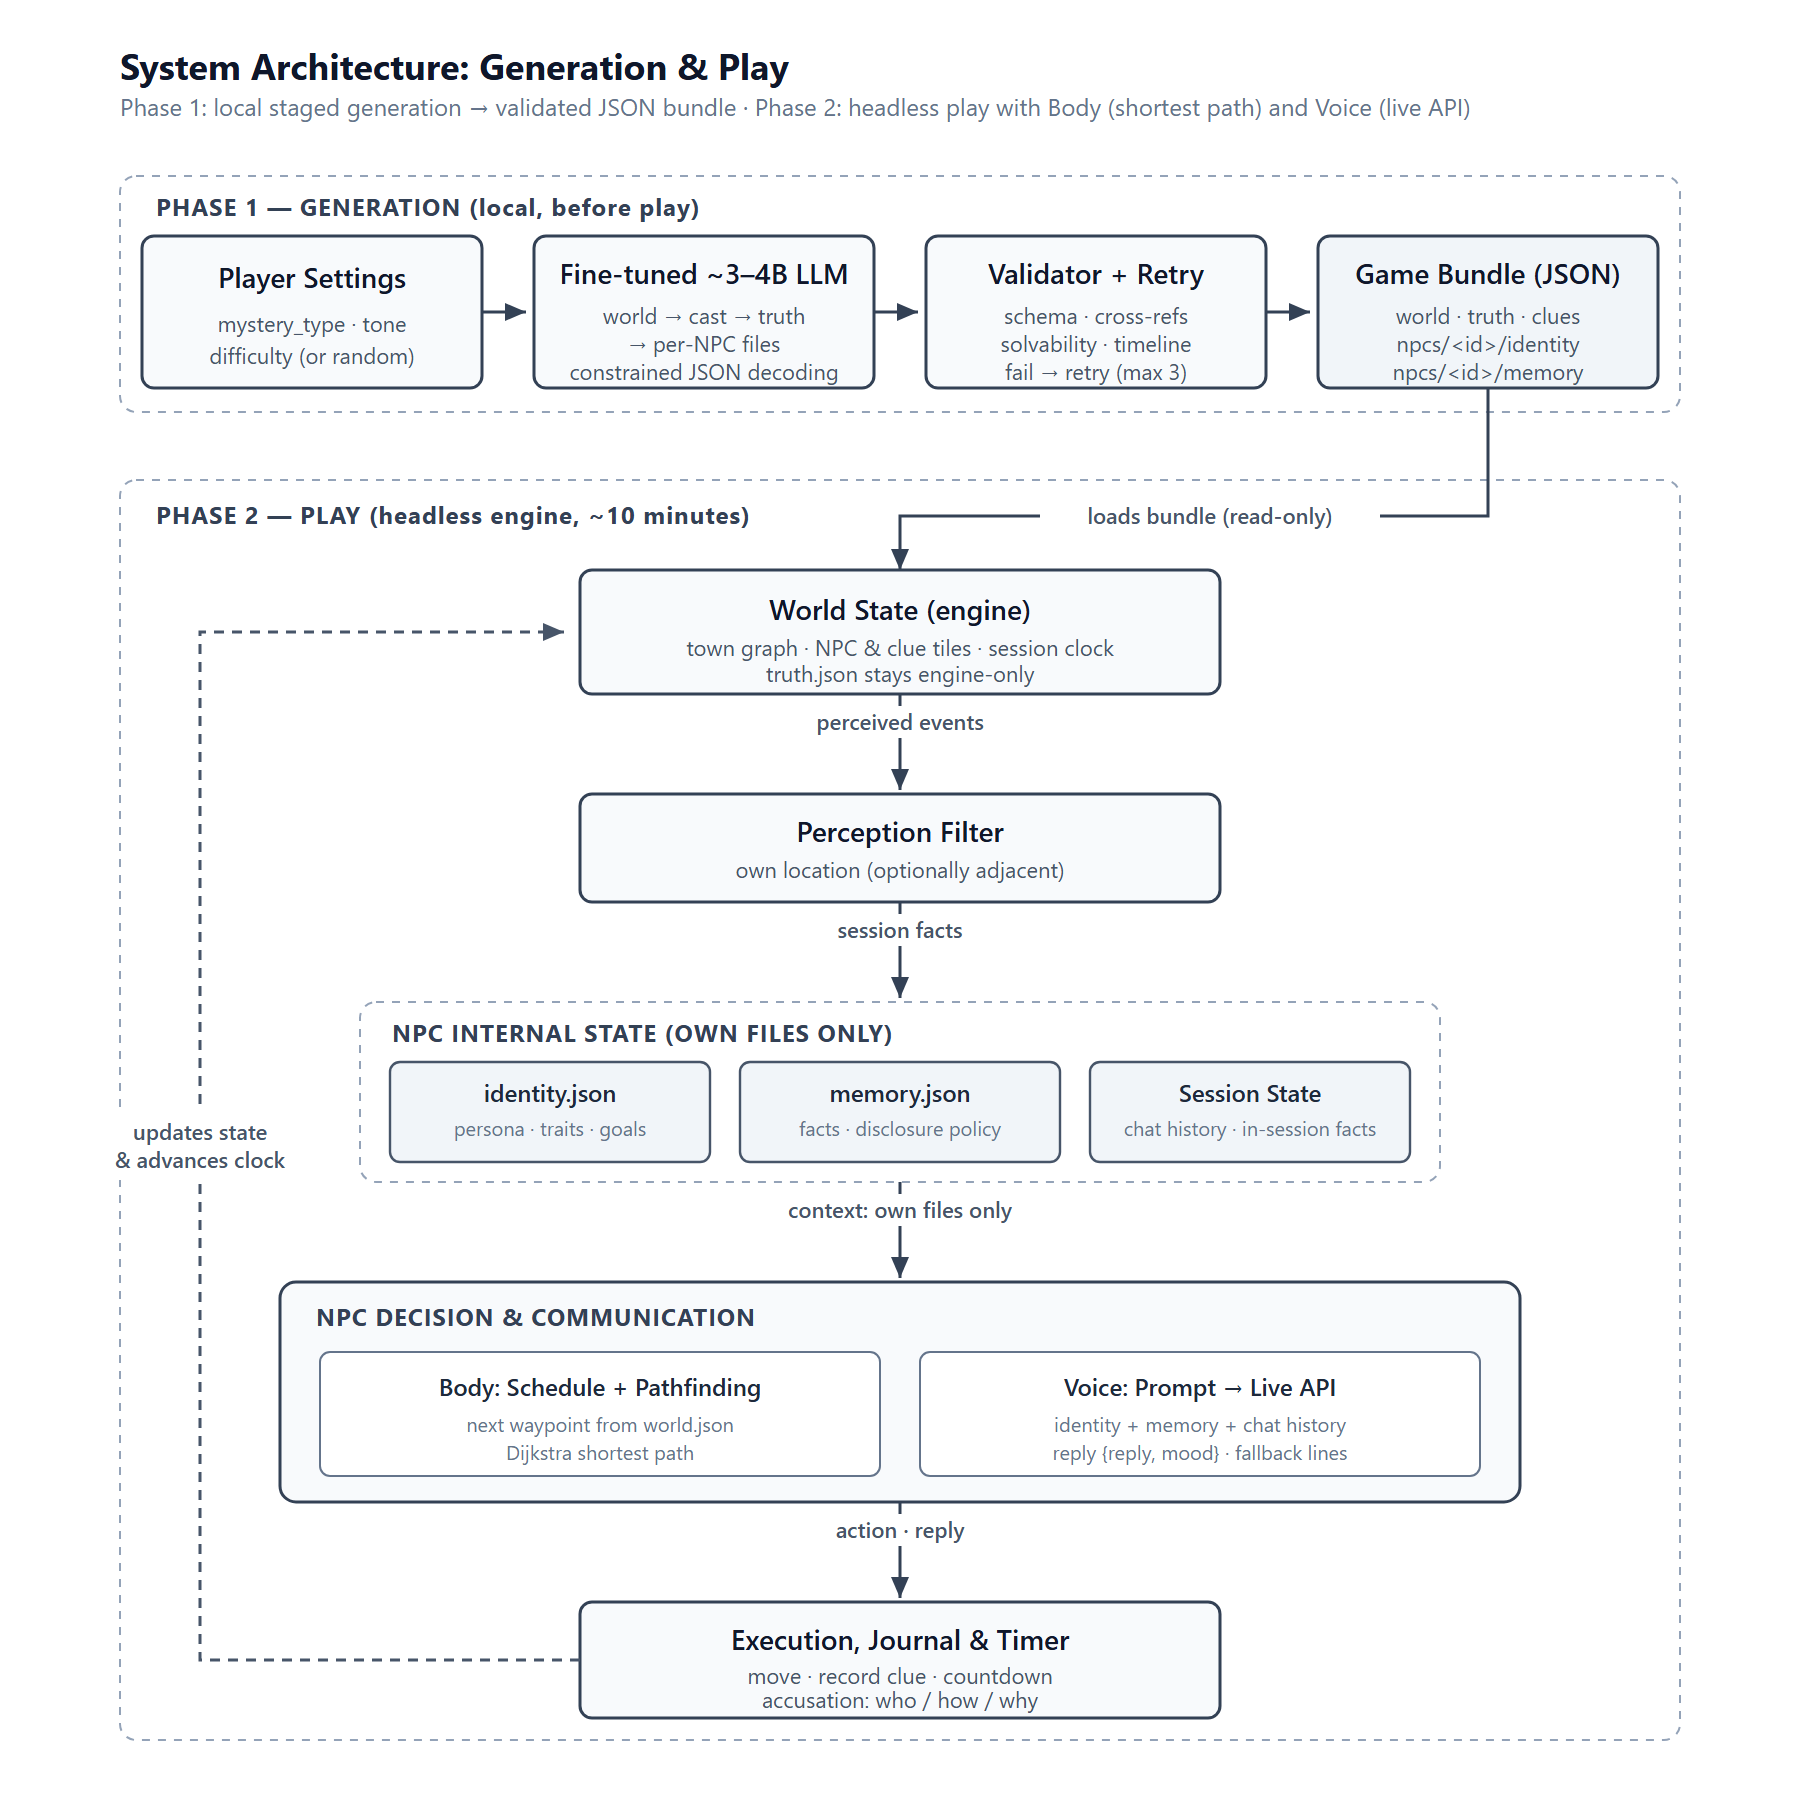
\includegraphics[width=\textwidth]{figures/system_architecture.png}
  \caption{The two-phase architecture. Phase~1 generates and validates the bundle offline; Phase~2 runs a headless simulation with a thin Pygame client. The engine is the sole holder of the truth file.}
  \label{fig:system}
\end{figure}

\section{The Body and the Voice}
The play phase separates two kinds of intelligence.

\textbf{The Body} is classical. It owns the world graph, the session clock, NPC schedules, shortest-path movement, proximity perception, clue discovery, the journal, and the accusation. It is pure Python with zero UI imports, so it can run headless in tests and in the evaluation harness. Its behaviour is predictable down to the tick, which is what makes a ten-minute deduction game testable.

\textbf{The Voice} is neural, but remote. When a player speaks to an NPC, a prompt assembler builds a request from that NPC's \texttt{identity.json}, \texttt{memory.json}, and the conversation so far. A live provider (Gemini or xAI) answers in character. If no key is configured, or the provider fails repeatedly, a deterministic authored fallback replies and reveals eligible clues. The fallback is not a degraded toy: it is the default offline path, and it keeps the game completable.

\begin{figure}[htbp]
  \centering
  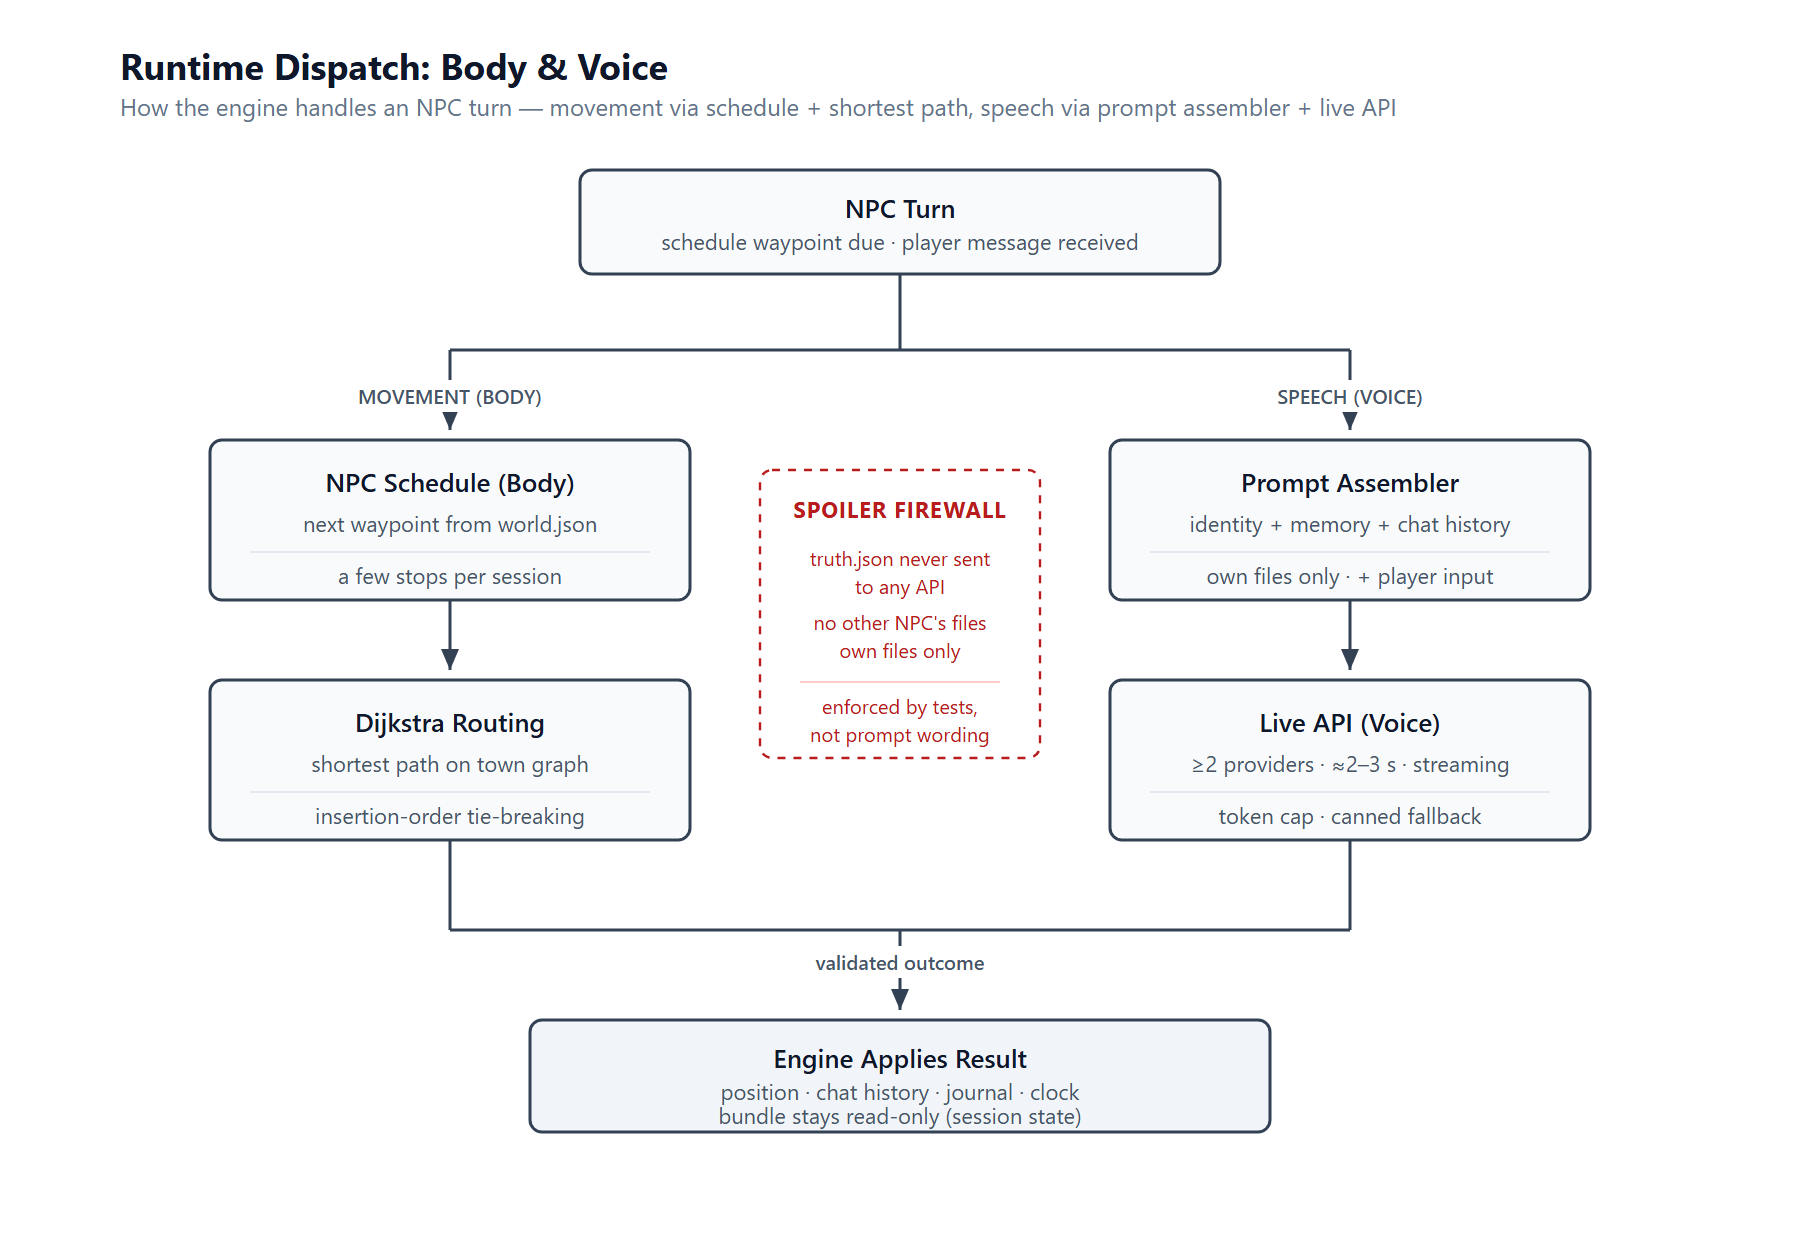
\includegraphics[width=0.86\textwidth]{figures/dispatch.png}
  \caption{Runtime dispatch. Movement follows a schedule and Dijkstra routing; speech follows the prompt assembler. The spoiler firewall sits between the two, enforced by tests rather than by prompt wording.}
  \label{fig:dispatch}
\end{figure}

\section{The Bundle Contract}
The generation phase produces a directory with a fixed shape:

\begin{lstlisting}[style=bundle]
case_dir/
  world.json                    # locations, NPC roster, schedules, accusation options
  truth.json                    # ENGINE-ONLY: culprit, method, motive, timeline
  clues.json                    # evidence, discovery method, implications
  npcs/<npc_id>/identity.json   # name, role, traits, backstory, speech style
  npcs/<npc_id>/memory.json     # facts the NPC knows, with disclosure policy
\end{lstlisting}

The schema is frozen at version 1.0 and implemented as Pydantic models \cite{pydantic}. Cross-file validation is stricter than per-file validation: references must resolve, the location graph must be connected, every NPC must have a schedule, the culprit must appear, and the clue set must satisfy the solvability condition. A bundle that fails any of these checks is never published.

\section{Design Principles}
Four principles recur throughout the implementation.

\begin{keybox}[Architecture in one sentence]
Let the model write the mystery; let the engine write the data structure; prove the case is solvable before the player sees it; and never let the solution enter a prompt.
\end{keybox}

\begin{enumerate}
  \item \textbf{Neural ideation, symbolic bookkeeping.} Models are good at premise, motive, and social texture, and bad at repetitive syntax and global consistency. The architecture assigns each to its strength.
  \item \textbf{Verify, then publish.} Validation and solvability are gates, not suggestions. Publication is atomic: a failed run leaves the previous bundle untouched.
  \item \textbf{Truth is engine-only.} \texttt{truth.json} is read by the accusation service and by validators. It is not part of any prompt, and the conversation service has no code path that could read it.
  \item \textbf{Graceful degradation.} Missing keys, provider timeouts, and absent model files all have deterministic fallbacks. The game remains playable offline, and the fallback path is excluded from live-provider metrics.
\end{enumerate}

\chapter{The Generation Pipeline}
\label{ch:generation}

\section{Overview}
Two generation routes share one output contract. The \emph{blueprint route} is the production path used by the game's ``Generate Locally'' option and by \texttt{python -m fabula generate --fast}. A 1B model emits a compact DSL sketch; a symbolic compiler expands it. The \emph{staged route} is the original path: a 3B model serialises the contract as JSON in several passes, with a JSON-schema grammar and per-stage retries. Both routes end at the same gate: Pydantic parsing, cross-file validation, solvability proof, and atomic publication.

\begin{figure}[htbp]
  \centering
  \begin{tikzpicture}[
      node distance=5mm and 6mm,
      every node/.style={font=\footnotesize\sffamily},
      stage/.style={draw=FNavy!55, thick, fill=FNavy!4, rounded corners=3pt,
        align=center, minimum height=12mm, text width=2.65cm, inner sep=3pt},
      gate/.style={draw=FGold!85!black, thick, fill=FGold!12, rounded corners=3pt,
        align=center, minimum height=12mm, text width=2.65cm, inner sep=3pt},
      arrow/.style={-{Latex[length=2mm]}, thick, draw=FNavy!65}
    ]
    \node[stage] (model) {Neural sketch\\[-1pt]{\scriptsize 1B model $\sim$150 DSL tokens}};
    \node[stage, right=of model] (parse) {Parse \& normalise\\[-1pt]{\scriptsize entities, minutes, links}};
    \node[stage, right=of parse] (compile) {Epistemic compiler\\[-1pt]{\scriptsize world, cast, memory}};
    \node[gate, right=of compile] (proof) {Solvability proof\\[-1pt]{\scriptsize candidates $=\{c\}$}};
    \node[gate, below=9mm of proof] (validate) {Schema \& cross-file\\[-1pt]{\scriptsize validation}};
    \node[gate, left=of validate] (publish) {Atomic publication\\[-1pt]{\scriptsize temp dir $\rightarrow$ rename}};
    \draw[arrow] (model) -- (parse);
    \draw[arrow] (parse) -- (compile);
    \draw[arrow] (compile) -- (proof);
    \draw[arrow] (proof) -- (validate);
    \draw[arrow] (validate) -- (publish);
    \node[draw=FCrimson!70, dashed, rounded corners=2pt, font=\scriptsize\sffamily,
          text=FCrimson, align=center, below=7mm of parse, text width=4.2cm]
      {semantic choices preserved;\\ structural gaps filled deterministically};
  \end{tikzpicture}
  \caption{The blueprint route. The model supplies narrative intent; parsing, compilation, proof, and publication are deterministic Python.}
  \label{fig:pipeline}
\end{figure}

\section{Why Syntax Is the Enemy}
Autoregressive decoding is memory-bandwidth bound. Every generated token streams the active weights through the CPU, so throughput scales roughly with model size and inversely with syntax overhead. The original staged route generated 3,245--3,656 output tokens per case, most of them JSON punctuation and repeated keys, at about five tokens per second. The blueprint route generates 243--299 tokens at about 31 tokens per second. The arithmetic is brutal and favourable: roughly twelve times fewer tokens at roughly six times the rate.

\begin{table}[htbp]
  \centering
  \small
  \begin{tabular}{@{}lrrr@{}}
    \toprule
    \textbf{Representation} & \textbf{Tokens} & \textbf{@ 30 tok/s} & \textbf{@ 5 tok/s} \\
    \midrule
    Staged JSON (9 passes) & $\sim$7{,}200 & not viable & $\sim$24 min \\
    Single JSON blueprint & $\sim$520 & 17.3 s & 104 s \\
    Compact blueprint DSL & $\sim$150 & 5.0 s & 30 s \\
    \midrule
    \textbf{Measured 1B DSL route (warm)} & \textbf{279} & \textbf{9.0 s} & --- \\
    \textbf{Measured 3B staged route} & \textbf{3{,}450} & --- & \textbf{657.7 s} \\
    \bottomrule
  \end{tabular}
  \caption{Token economics. Measured rows come from the evaluation recorded in Chapter~\ref{ch:eval}; projection rows illustrate the design arithmetic from the architecture specification.}
  \label{tab:tokens}
\end{table}

\section{Route A: The Compact Blueprint DSL}
The DSL is line-oriented and deliberately terse. A complete sketch contains a case header, a premise, a cast, a crime, a timeline, clues, and optional knowledge lines. The following is a representative example (the actual model output is shorter and less tidy):

\begin{lstlisting}[style=dsl]
[CASE:theft|cozy|hard|seed_101]
PREMISE: A silver locket vanishes from the Old Library during the evening reading.
CAST: vict:lady_eleanor | culp:npc_butler | susp:npc_maid,npc_gardener,npc_nephew
CRIME: mot:gambling_debt | meth:skeleton_key | scene:loc_library | time:5
TIMELINE:
- 2 | npc_butler | loc_cafe | retrieves duplicate brass key
- 4 | npc_maid | loc_market | delivers tea service
- 5 | npc_butler | loc_library | unlocks display cabinet and takes the locket
- 7 | npc_nephew | loc_park | sees the butler walking away quickly
CLUES:
- brass_shaving | loc_library | physical | links:npc_butler | proves:meth
- debt_ledger | loc_cafe | document | links:npc_butler | proves:mot
- muddy_glove | loc_park | trace | red_herring:npc_gardener
KNOWLEDGE:
- npc_maid | sees:butler_near_cabinet | alibi:in_market_at_minute_5
- npc_nephew | sees:butler_in_park | alibi:in_park_with_gardener
\end{lstlisting}

The compiler accepts variation. It tolerates missing optional fields, human-readable prose in the premise, and cast names that do not match the final identifiers. What it does not tolerate is a fatal contradiction: a crime scene outside the map, a culprit missing from the cast, or a timeline that cannot be ordered.

\subsection{Compilation Steps}
The compiler performs the following stages, in order:

\begin{enumerate}
  \item \textbf{Parse} the header, premise, cast, crime, timeline, clues, and knowledge lines into an internal blueprint object.
  \item \textbf{Normalise} identifiers, resolve cast references, clamp minutes to the ten-minute window, and map unnamed locations onto the available location types.
  \item \textbf{Build the world}: place four connected locations, assign the cast to the roster, and derive a small set of schedule waypoints from the timeline.
  \item \textbf{Build the truth}: fix the culprit, method, motive, scene, and minute exactly as the model wrote them. The compiler never reassigns the culprit.
  \item \textbf{Authored clues}: turn each clue line into a clue with a location, a discovery method, an implication list, and optional requirements.
  \item \textbf{Epistemic slicing}: derive each NPC's facts from the timeline using strict provenance. An innocent knows events they performed or directly observed; the culprit additionally receives the true account as a secret, plus an authored cover story.
  \item \textbf{Fill structural gaps}: if the sketch lacks a required clue type, an accusation option, or a schedule entry, synthesise it from the model's own cast and timeline.
  \item \textbf{Prove solvability} and reject the bundle if the candidate set does not collapse to the culprit.
  \item \textbf{Publish atomically} after Pydantic and cross-file validation succeed.
\end{enumerate}

The distinction between \emph{semantic} and \emph{structural} content is the key to the design. If the model says the culprit is the butler, the compiler makes the butler the culprit. If the model forgets to give the butler an alibi claim, the compiler may add one; it may not change who did it.

\section{Route B: Staged JSON}
The staged route predates the blueprint work and remains useful as a comparison. It generates the bundle in four logical passes: settings and world, then cast, then truth and clues, then one identity/memory pair per NPC. Each pass is constrained by a JSON-schema grammar compiled from the frozen Pydantic models, with two llama.cpp-specific safeguards. First, pattern and length constraints are removed from the grammar because \texttt{maxLength} expands into nested groups that exceed the grammar compiler's depth limit; Pydantic still enforces them after parsing. Second, NPC-stage identifiers are pinned with enums so a model cannot assign one character's memory to another.

Two final repairs run after all stages. If the culprit has no secret \texttt{did} fact, the engine adds one from the truth file. If no clue implies a culprit-owned fact, the crime-scene clue is linked to the culprit's account. These repairs guarantee a playable case, but they also reveal the core weakness of the staged route: the model is asked to maintain global consistency across thousands of tokens, and the engine has to repair the result after the fact.

\begin{warnbox}[Why the staged route is no longer the default]
The staged route is valid and expressive, but it is not a ten-minute-game generator. On the measured machine it took 657.7\,s on average for two valid runs, failed validation once in three attempts, and required over 3.4\,GB of RAM. The blueprint route is 72.8 times faster at roughly 1.5\,GB. The staged route is retained for comparison and as a source of teacher data, not as the shipping path.
\end{warnbox}

\section{Solvability}
\label{sec:solvability}
Let $F$ be the set of facts, $C$ the clue set, and $\mathit{implies}(c)\subseteq F$ the facts a clue supports. Let $\mathit{owner}(f)$ be the NPC who owns fact $f$. The compiler checks two conditions:

\begin{align}
  \{\, \mathit{owner}(f) : f \in \textstyle\bigcup_{c\in C}\mathit{implies}(c),\ f.\mathit{source}=\text{did},\ f.\mathit{secret}=\text{true} \,\} &= \{\, \mathit{culprit} \,\}, \\
  \forall\, i \in \mathit{innocents}:\quad \exists\, c\in C,\ f\in\mathit{implies}(c) &: \ f=\mathit{alibi}_i .
\end{align}

The first condition says that the only person who owns a clue-reachable secret deed is the culprit. The second says that every innocent has an alibi fact reachable from some clue. Together they implement candidate elimination: a player who finds the relevant clues can rule everyone else out. The proof is deliberately conservative. It does not claim that every generated clue is \emph{interesting}, only that the solution is reachable.

\section{Atomic Publication and Integrity}
Generation writes to a temporary sibling directory. Only after the complete bundle passes validation and the solvability proof is the directory renamed into place. A crash, a validation failure, or a rejected proof leaves any previous bundle untouched. The published directory is content-addressable in practice: evaluation records hash the model files, and the corpus records an integrity hash over all generated skeletons. This makes runs comparable and makes silent corruption visible.

\chapter{Data and Model Training}
\label{ch:data}

\section{The Skeleton Corpus}
Training begins with structured skeletons rather than finished prose. A skeleton fixes the scenario type, tone, difficulty, cast size, location graph, clue count, and disclosure facts. We generated 300 skeletons, exactly 100 each of theft, disappearance, and murder, with a balanced tone distribution (101 cozy, 99 dark, 100 neutral). The generator enforces a set of invariants before a skeleton is accepted: every location is reachable, every NPC has a schedule, every secret has an owner, and every scenario has one culprit. The cleaning report records zero rejected and zero duplicate scenarios, and the corpus is sealed with an integrity hash.

\begin{figure}[htbp]
  \centering
  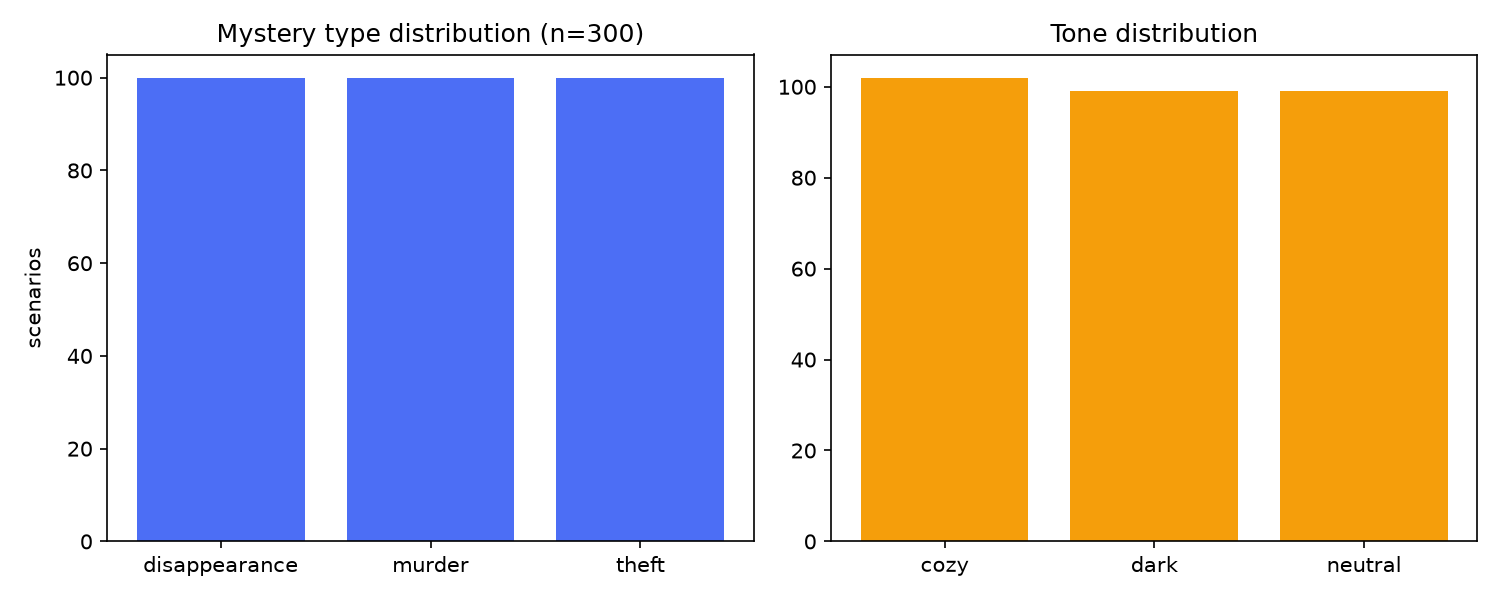
\includegraphics[width=0.95\textwidth]{figures/eda_class.png}
  \caption{Corpus balance. The 300 skeletons are stratified by mystery type and tone so that neither the teacher nor the student sees a skewed prior.}
  \label{fig:eda}
\end{figure}

\begin{figure}[htbp]
  \centering
  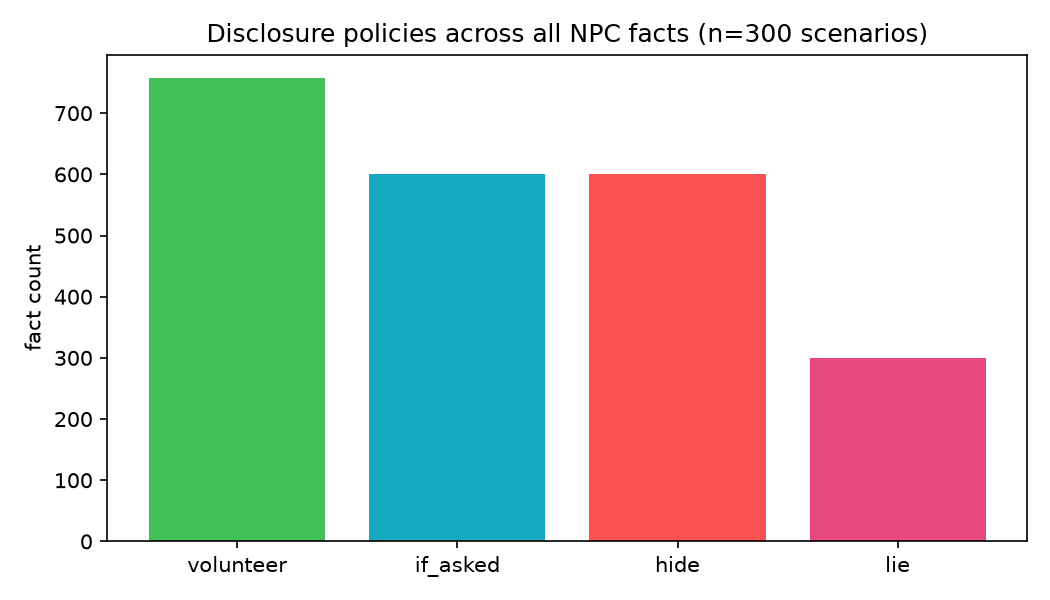
\includegraphics[width=0.72\textwidth]{figures/eda_disclosure.png}
  \caption{Disclosure policies across all NPC facts. Roughly half the facts are volunteered, a third are available only if asked, and a smaller set are hidden or actively lied about. The distribution gives the dialogue layer something to protect.}
  \label{fig:disclosure}
\end{figure}

The skeletons are intentionally not mystery plots. They are grounded configurations: who is present, where they can be, what kinds of secrets exist, and which disclosure policy applies. The teacher model's job is to turn a configuration into a coherent case. Splitting is done by seed, not by row, so near-duplicate paraphrases of the same underlying configuration cannot leak across train and test.

\section{Teacher Expansion}
We used Qwen2.5-7B-Instruct in FP16 on Kaggle's dual Tesla T4 environment as the teacher. The run is a batched enrichment pass, not a fine-tune: the teacher reads each clean skeleton and writes a rich case, including location descriptions, character texture, and clue prose. The console captures in Figure~\ref{fig:teacher} document the operational reality: a 112.4-second model load, 13.4 tokens/s for a single inference, and a 991.0-second batched pass over all 300 skeletons at batch size eight.

\begin{figure}[htbp]
  \centering
  \begin{subfigure}[t]{0.48\textwidth}
    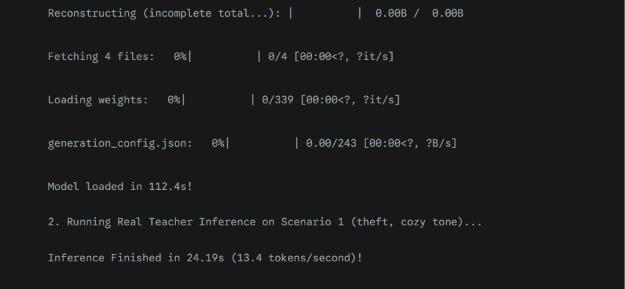
\includegraphics[width=\linewidth]{figures/teacher_loaded.jpg}
    \caption{Model load and first inference.}
    \label{fig:teacher-load}
  \end{subfigure}\hfill
  \begin{subfigure}[t]{0.48\textwidth}
    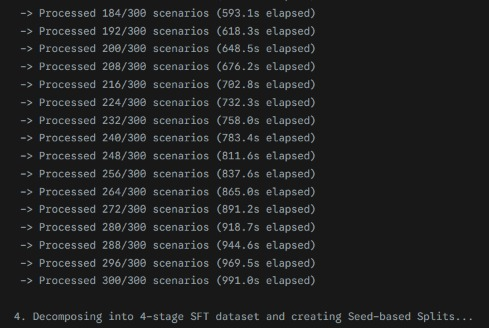
\includegraphics[width=\linewidth]{figures/teacher_done.jpg}
    \caption{Batched enrichment completes 300/300 skeletons in 991.0\,s.}
    \label{fig:teacher-done}
  \end{subfigure}
  \caption{Teacher expansion on dual Tesla T4s. The 7B model enriches skeletons into complete cases; this stage produces the supervised data, not the runtime artefact.}
  \label{fig:teacher}
\end{figure}

The enrichment produced 2,558 supervised pairs, split 2,048 for training, 256 for validation, and 254 for test. The teacher's output is not trusted blindly: every case still passes the same structural validators used by the runtime. A teacher that writes a beautiful but unsolvable case produces a rejected sample, not a training pair.

\begin{figure}[htbp]
  \centering
  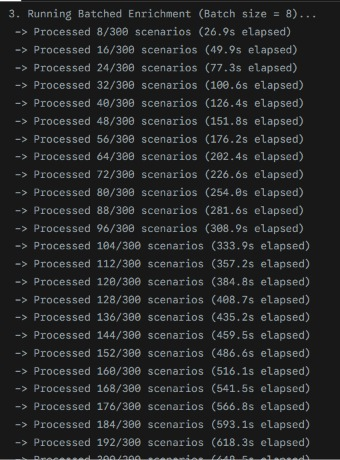
\includegraphics[width=0.7\textwidth]{figures/teacher_batch.jpg}
  \caption{Batched enrichment progress. Batch size eight keeps both T4s busy without exhausting memory.}
  \label{fig:teacher-batch}
\end{figure}

\section{Staged 3B QLoRA}
The staged route fine-tunes Qwen2.5-3B-Instruct. The base model is loaded in four-bit precision with Unsloth, and LoRA adapters are attached to the attention and MLP projections (rank 16, $\alpha=16$, no dropout). Training uses a maximum sequence length of 2,560, response-only loss masking, two epochs, a learning rate of $2\times10^{-4}$ with a cosine schedule, 15 warm-up steps, an effective batch size of eight (two per device times four accumulation steps), and \texttt{adamw\_8bit} with weight decay 0.01. The run completed 512 steps in about 2 hours 45 minutes on a single T4.

\begin{figure}[htbp]
  \centering
  \begin{subfigure}[t]{0.48\textwidth}
    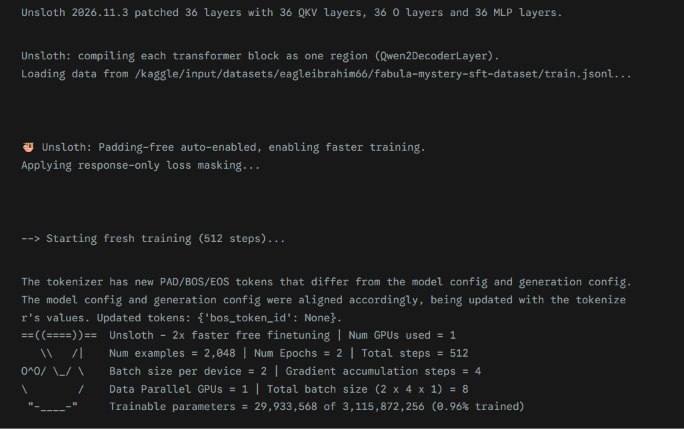
\includegraphics[width=\linewidth]{figures/qwen_start.jpg}
    \caption{Unsloth patches the model and loads the 2,048-example training set.}
    \label{fig:qwen-start}
  \end{subfigure}\hfill
  \begin{subfigure}[t]{0.48\textwidth}
    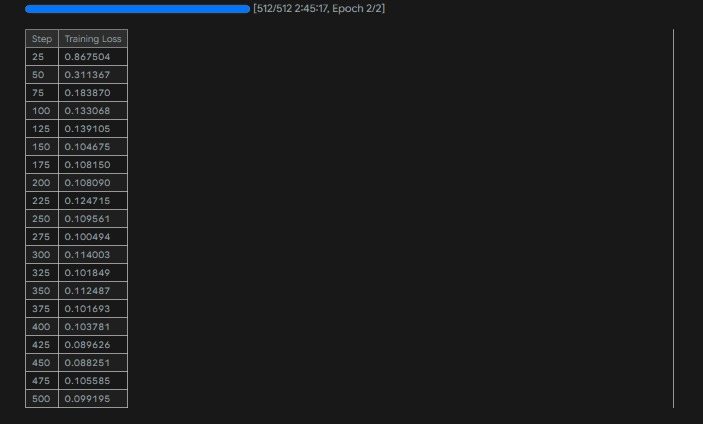
\includegraphics[width=\linewidth]{figures/qwen_loss.jpg}
    \caption{Training loss falls from 0.868 at step 25 to 0.099 at step 500.}
    \label{fig:qwen-loss}
  \end{subfigure}
  \caption{Staged 3B QLoRA training. Response-only masking means the loss is computed on the assistant JSON, not on the prompt.}
  \label{fig:qwen}
\end{figure}

\begin{figure}[htbp]
  \centering
  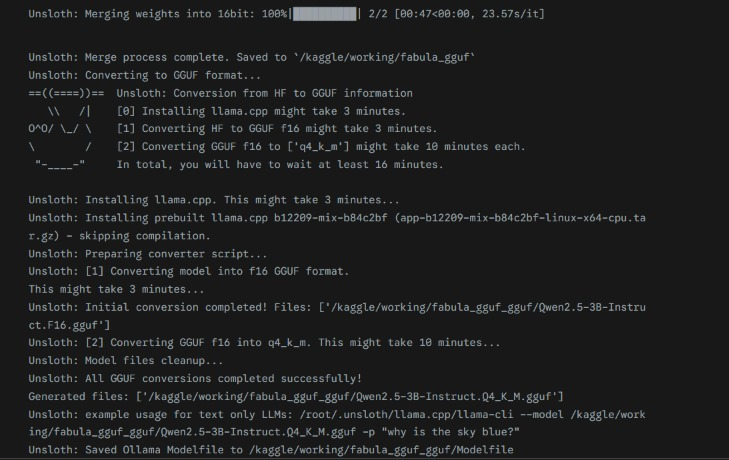
\includegraphics[width=0.72\textwidth]{figures/qwen_gguf.jpg}
  \caption{Merge and quantisation. The adapter is merged into 16-bit weights and converted to GGUF Q4\_K\_M; the resulting artefact is 1.93\,GB and is verified against the model manifest by SHA-256.}
  \label{fig:qwen-gguf}
\end{figure}

\section{Blueprint Distillation and the 1B Student}
The 1B student never sees the staged JSON. It is trained on blueprint sketches produced by the teacher and checked by the compiler. We generated 1,500 DSL samples with disjoint seeds, split 1,200/150/150 into train, validation, and test. The student is Llama-3.2-1B-Instruct loaded in four-bit precision, with the same rank-16 LoRA configuration, a maximum sequence length of 1,024, response-only masking, two epochs, a learning rate of $2\times10^{-4}$, cosine scheduling, 20 warm-up steps, and an effective batch size of eight (four per device times two accumulation steps). Training took roughly 35 minutes on one T4. The console captures in Figures~\ref{fig:llama} and~\ref{fig:llama-export} record the run: 11.27 million trainable parameters (0.90\% of the model), 300 optimizer steps, and a final training loss of 0.028. The adapter is then merged and quantised to Q4\_K\_M.

\begin{figure}[htbp]
  \centering
  \begin{subfigure}[t]{0.48\textwidth}
    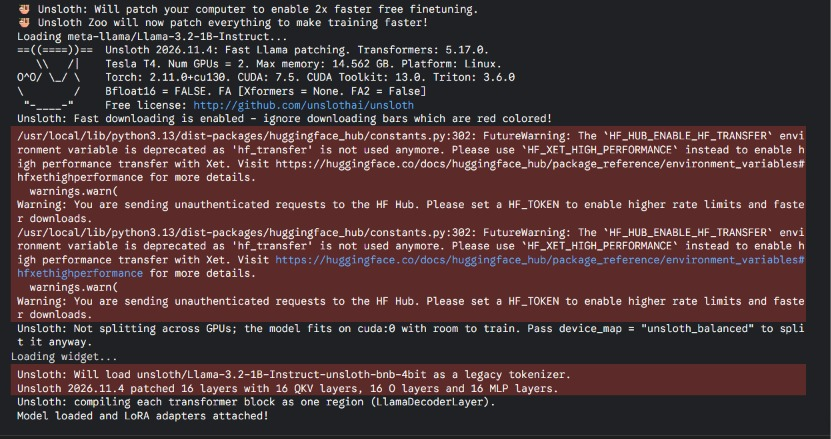
\includegraphics[width=\linewidth]{figures/llama_load.jpg}
    \caption{Loading the 1B base. Unsloth patches Llama-3.2-1B-Instruct and attaches the LoRA adapters.}
    \label{fig:llama-load}
  \end{subfigure}\hfill
  \begin{subfigure}[t]{0.48\textwidth}
    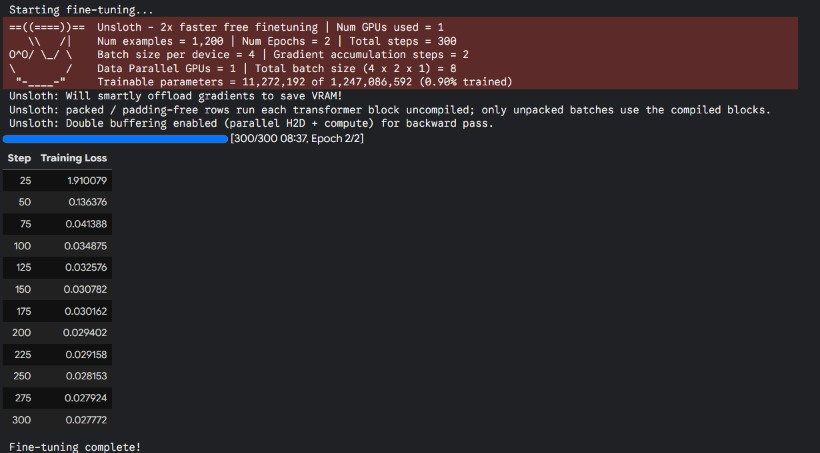
\includegraphics[width=\linewidth]{figures/llama_train.jpg}
    \caption{Training the 1B student. The run covers 1,200 examples in 300 steps; loss falls to 0.028.}
    \label{fig:llama-loss}
  \end{subfigure}
  \caption{Blueprint distillation of the 1B student. Only 0.90\% of the parameters are trainable; the run completes in about 35 minutes on one T4.}
  \label{fig:llama}
\end{figure}

\begin{figure}[htbp]
  \centering
  \begin{subfigure}[t]{0.48\textwidth}
    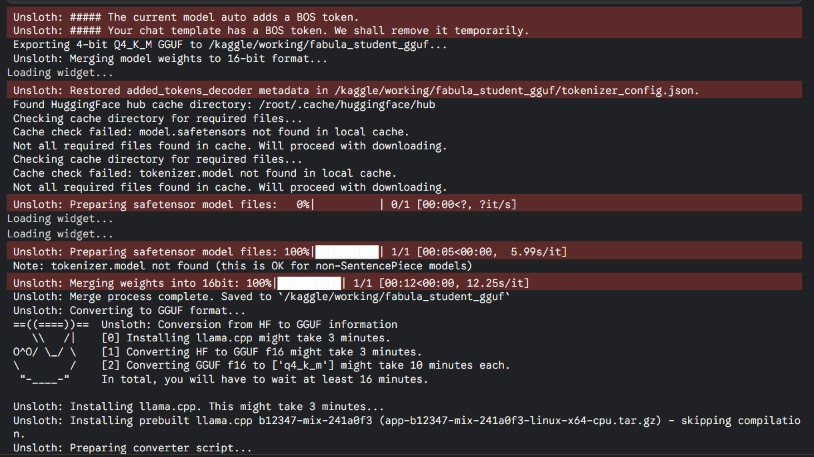
\includegraphics[width=\linewidth]{figures/llama_merge.jpg}
    \caption{Merging the adapter into 16-bit weights before quantisation.}
    \label{fig:llama-merge}
  \end{subfigure}\hfill
  \begin{subfigure}[t]{0.48\textwidth}
    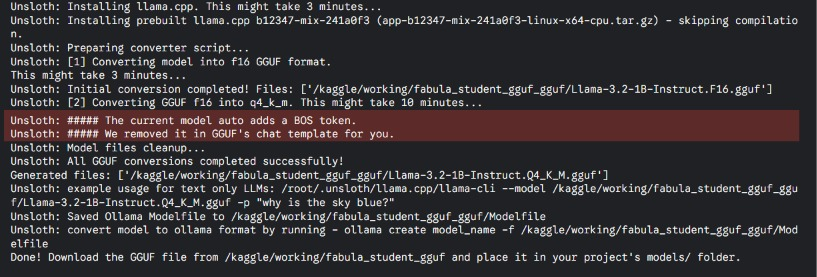
\includegraphics[width=\linewidth]{figures/llama_gguf.jpg}
    \caption{GGUF conversion. The pipeline writes an F16 checkpoint and a Q4\_K\_M file for the runtime.}
    \label{fig:llama-gguf}
  \end{subfigure}
  \caption{Export of the 1B student. The Q4\_K\_M GGUF is the artefact loaded by the game runtime.}
  \label{fig:llama-export}
\end{figure}

\begin{table}[htbp]
  \centering
  \small
  \setlength{\tabcolsep}{4pt}
  \begin{tabular}{@{}>{\raggedright\arraybackslash}p{2.7cm}>{\raggedright\arraybackslash}p{3.4cm}>{\raggedright\arraybackslash}p{4.6cm}>{\raggedright\arraybackslash}p{3.2cm}@{}}
    \toprule
    \textbf{Stage} & \textbf{Base model} & \textbf{Key settings} & \textbf{Output} \\
    \midrule
    Teacher expansion & Qwen2.5-7B-Instruct (FP16) & batch 8, 300 skeletons, greedy-free sampling & 2,558 SFT pairs \\
    3B staged SFT & Qwen2.5-3B-Instruct (4-bit) & seq 2,560; $r{=}16$, $\alpha{=}16$; 2 epochs; 512 steps; lr $2\text{e-}4$ & Q4\_K\_M, 1.93\,GB \\
    DSL distillation & Qwen2.5-3B (teacher) & 1,500 seeds; compiler-verified & 1,200/150/150 split \\
    1B blueprint SFT & Llama-3.2-1B-Instruct (4-bit) & seq 1,024; $r{=}16$, $\alpha{=}16$; 2 epochs; lr $2\text{e-}4$ & Q4\_K\_M GGUF \\
    \bottomrule
  \end{tabular}
  \caption{Training and data stages. The two students are trained for different output contracts: staged JSON for the 3B route and compact DSL for the 1B route.}
  \label{tab:training}
\end{table}

\section{Export and Artifact Management}
Both students are exported to GGUF and quantised to Q4\_K\_M. The model files are intentionally excluded from version control; only a manifest with filename, base model, quantisation, license, and SHA-256 is committed. A CLI check recomputes the hash and fails hard on a mismatch. This matters for reproducibility: an evaluation that does not identify the exact weights is an anecdote, not a measurement.

\chapter{The Play Engine}
\label{ch:play}

\section{Deterministic Simulation}
The engine is a headless Python core with no UI imports. A session owns a clock, a loaded bundle, a clue index, a journal, an accusation service, and per-NPC records of what the player has said. The clock advances in real time during play views and pauses outside them, so opening the journal does not consume the ten-minute budget. NPCs follow short schedules expressed as waypoints in \texttt{world.json}; movement between waypoints uses Dijkstra's algorithm on the town graph with deterministic insertion-order tie-breaking. Perception is proximity-based, and events are appended to a session log.

This design has two benefits. First, it is testable: the entire play loop can be driven headlessly, with assertions about clue discovery, time-outs, accusation attempts, and NPC positions. Second, it is fair: the same bundle and the same inputs produce the same world state. The only non-deterministic component is live dialogue, and the scripted fallback exists precisely so that even that can be made deterministic.

\section{Knowledge Isolation and the Spoiler Firewall}
Each NPC's \texttt{memory.json} is a list of facts, not a prose summary. A fact has an owner, a kind, a source, a secrecy flag, and a disclosure policy. Innocent NPCs know only what they did or directly observed; alibis are checked against the spatial graph so that an NPC cannot be in two places at once. The culprit receives the true account as a secret fact with disclosure \texttt{lie}, plus an authored cover story explaining their presence elsewhere, plus motive and trace facts marked \texttt{hide}.

At runtime the prompt assembler reads only that NPC's identity, memory, and chat history. The truth file is not filtered out of a shared template; it is simply not part of the data the assembler can reach. The boundary is enforced by automated tests that plant canary strings in the truth file and assert they never appear in an outbound request.

\begin{figure}[htbp]
  \centering
  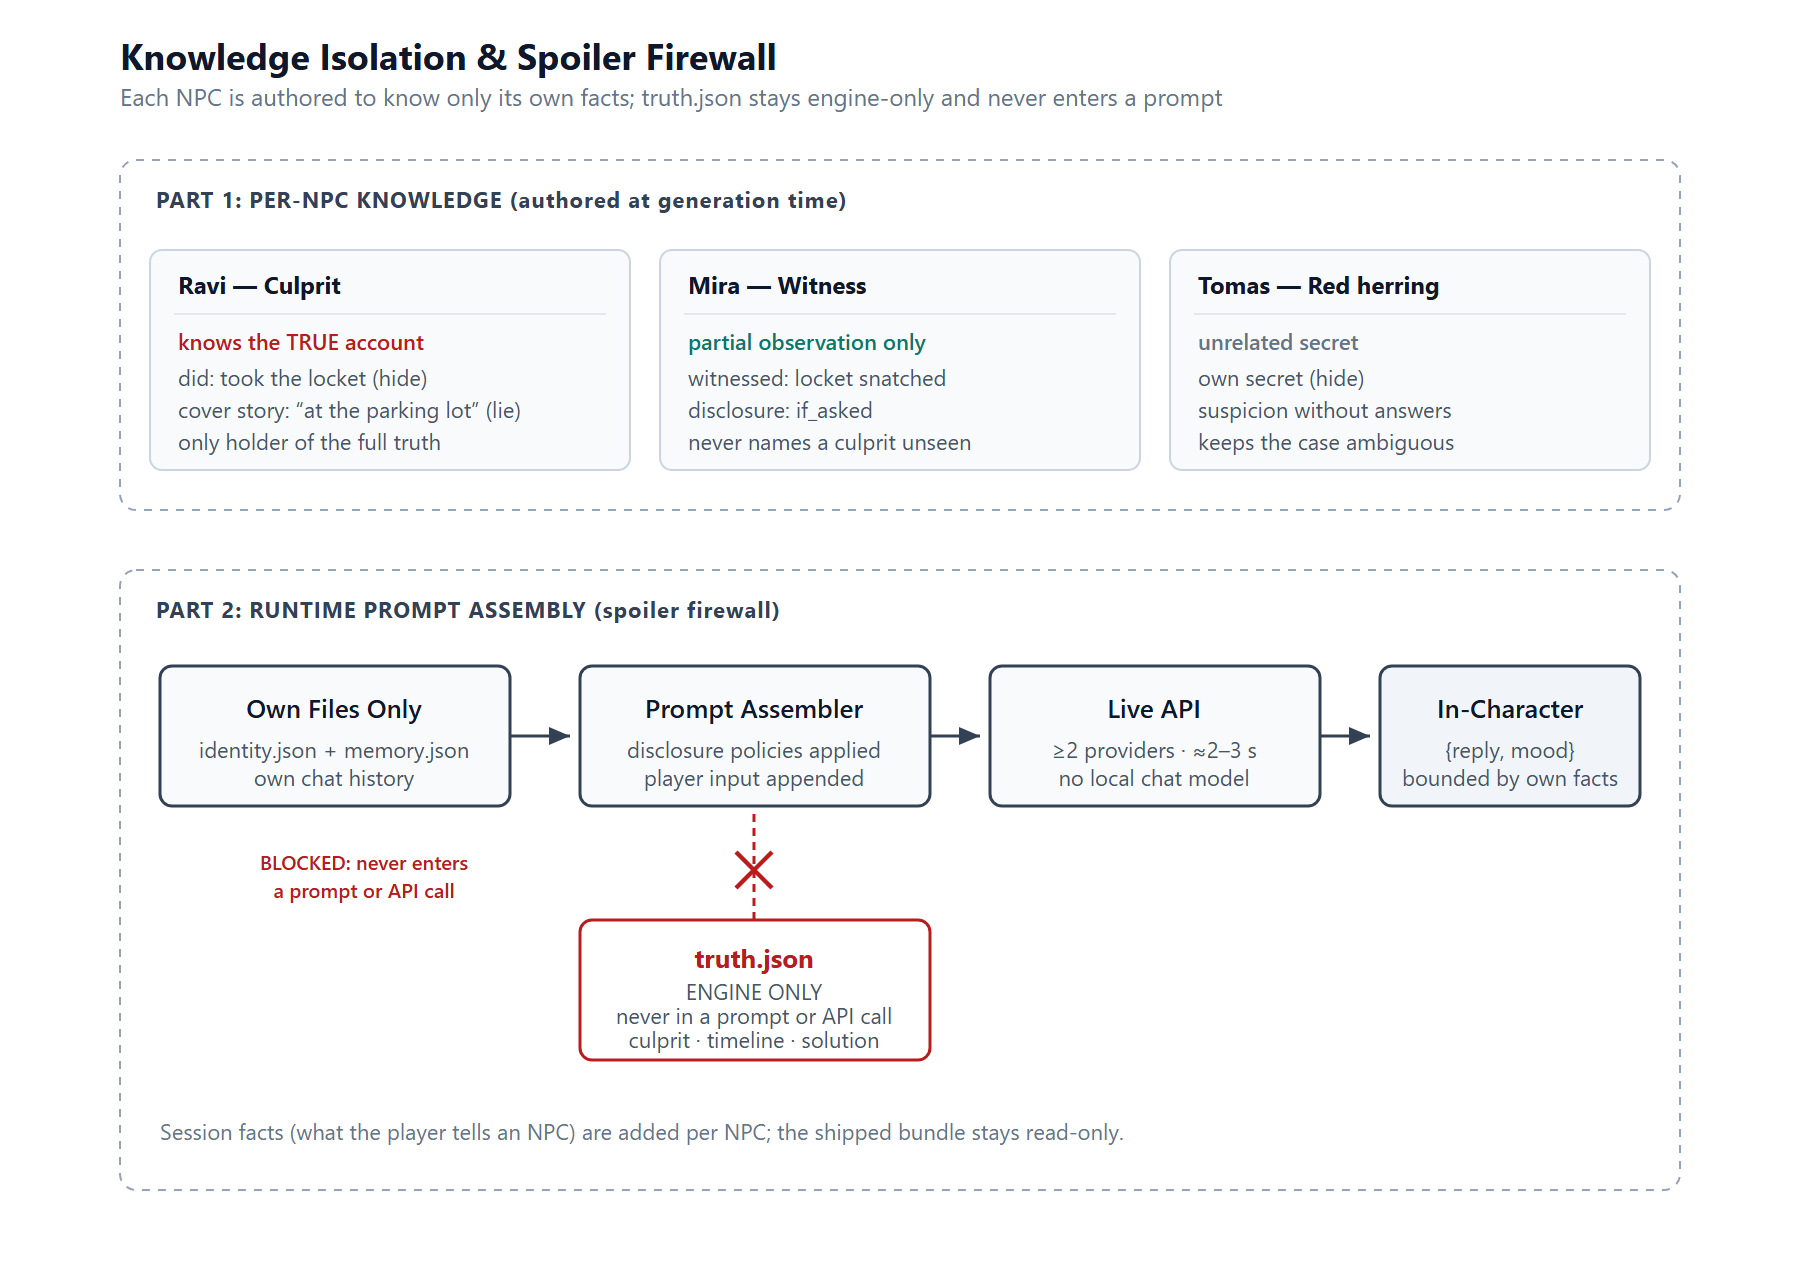
\includegraphics[width=\textwidth]{figures/knowledge_diffusion.png}
  \caption{Knowledge isolation. The culprit knows the true account; the witness holds a partial observation; the red herring holds an unrelated secret. At runtime, only the speaking NPC's own files reach the prompt assembler; the truth file never does.}
  \label{fig:knowledge}
\end{figure}

\section{Conversation}
The conversation service supports at least two live providers (Gemini and xAI) behind a common interface. A reply has a small schema: reply text, mood, and optional revealed clue IDs. The service enforces timeout budgets, per-session token caps, and a leak filter. When a provider fails, the NPC degrades to the authored scripted responder, which follows the same disclosure policy and can reveal eligible clues. The fallback is excluded from live-provider metrics, so provider comparisons are not contaminated by a deterministic baseline.

The prompt is intentionally narrow. It contains the NPC's identity and traits, the facts they know with their disclosure policies, and the recent conversation. It does not contain the town's truth, other NPCs' memories, or engine internals. This is both a security property and a behavioural one: an NPC cannot leak what they were never given, and their answers stay bounded by their own knowledge.

\section{Interface}
The client is a thin Pygame \cite{pygame} layer over the engine. It renders the illustrated town map, NPC portraits, the dialogue screen, the investigation journal, and the accusation board. The UI never mutates the bundle; session state lives in the engine. The result is a clean separation: the same engine can be driven by the desktop client, by the test suite, or by the evaluation harness.

\begin{figure}[htbp]
  \centering
  \begin{subfigure}[t]{0.49\textwidth}
    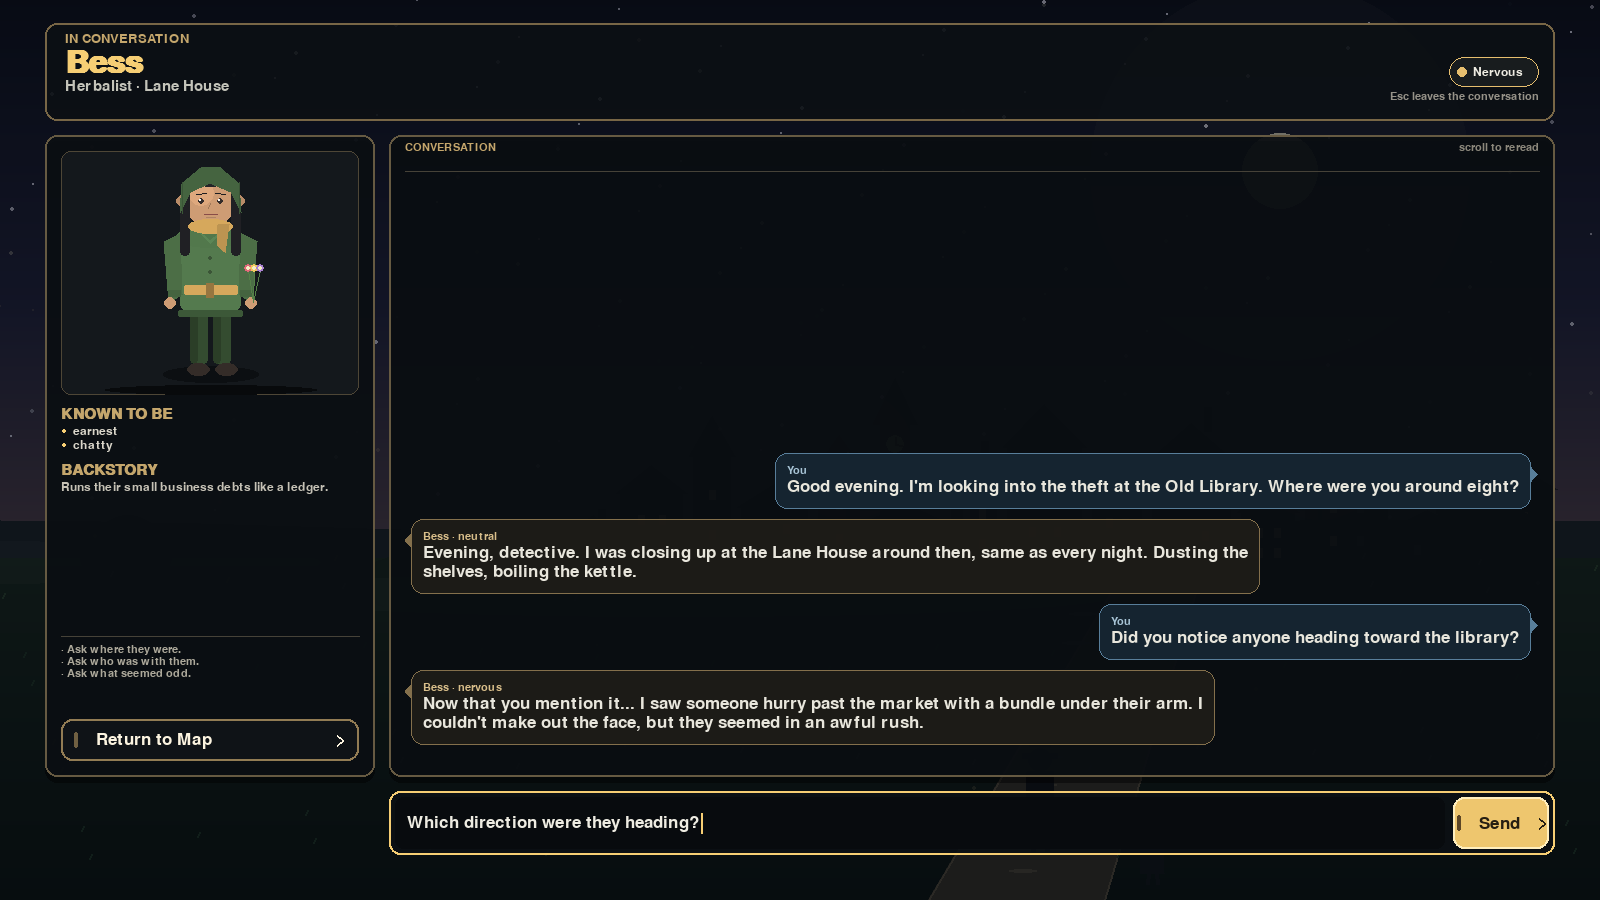
\includegraphics[width=\linewidth]{figures/dialogue.png}
    \caption{Dialogue. The sidebar shows only what this NPC is willing to share; the mood pill reflects the last reply.}
    \label{fig:dialogue}
  \end{subfigure}\hfill
  \begin{subfigure}[t]{0.49\textwidth}
    
\includegraphics[width=\linewidth]{figures/journal.png}
    \caption{Journal. Clues record where and when they were found; witness notes record what the player asked.}
    \label{fig:journal}
  \end{subfigure}
  \caption{The two core play screens.}
  \label{fig:playscreens}
\end{figure}

\begin{figure}[htbp]
  \centering
  \begin{subfigure}[t]{0.49\textwidth}
    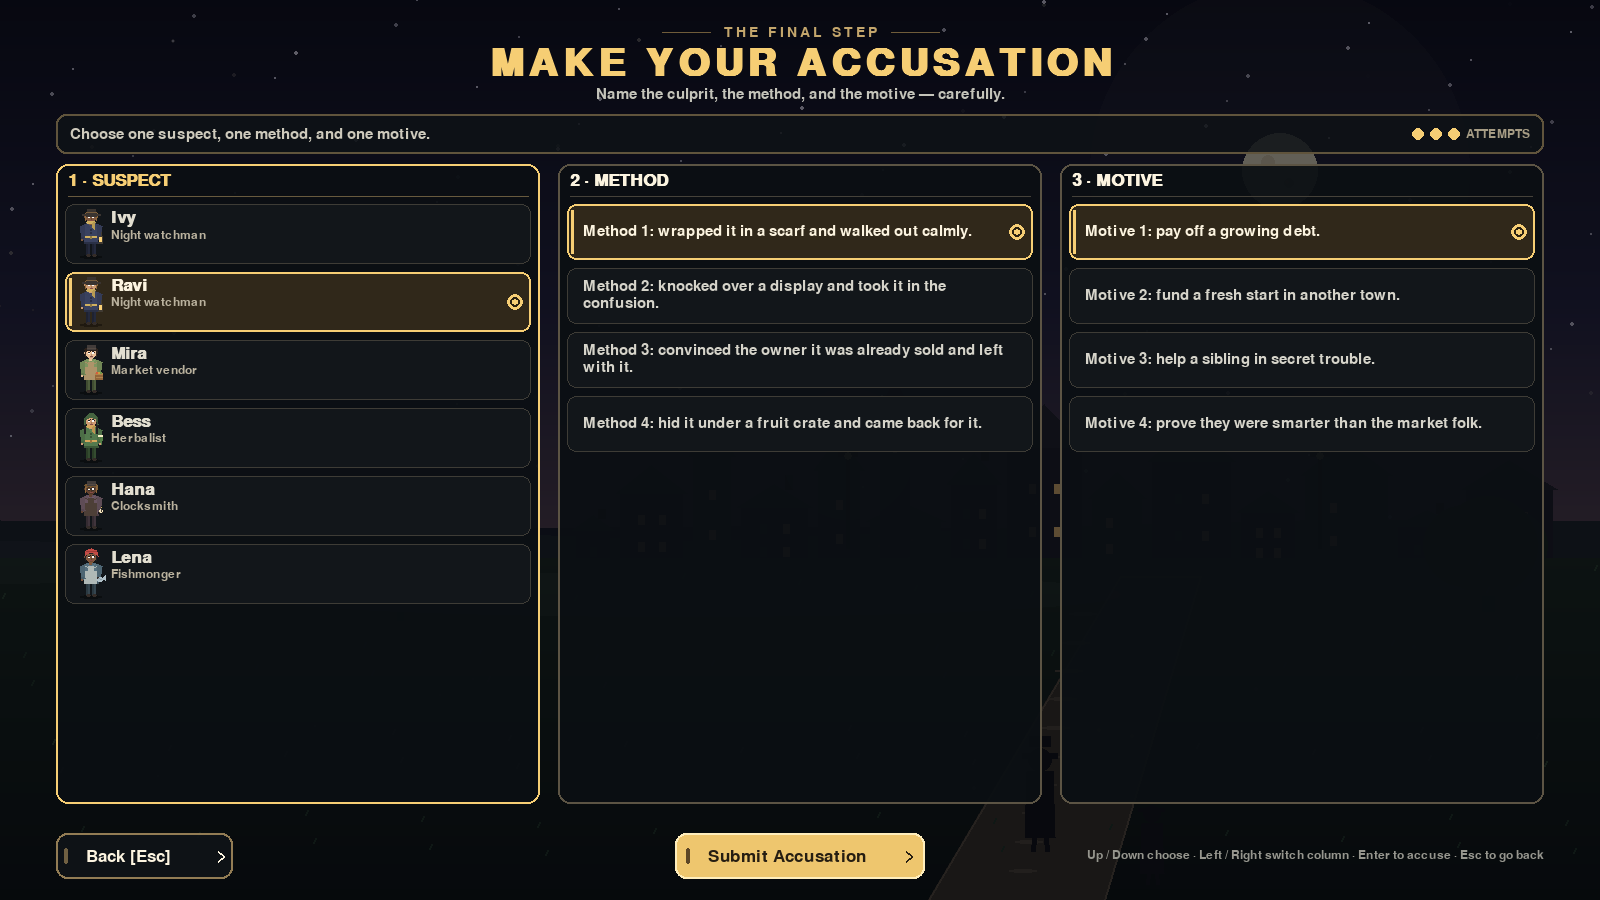
\includegraphics[width=\linewidth]{figures/accusation.png}
    \caption{The accusation board. The player chooses a suspect, a method, and a motive.}
    \label{fig:accusation}
  \end{subfigure}\hfill
  \begin{subfigure}[t]{0.49\textwidth}
    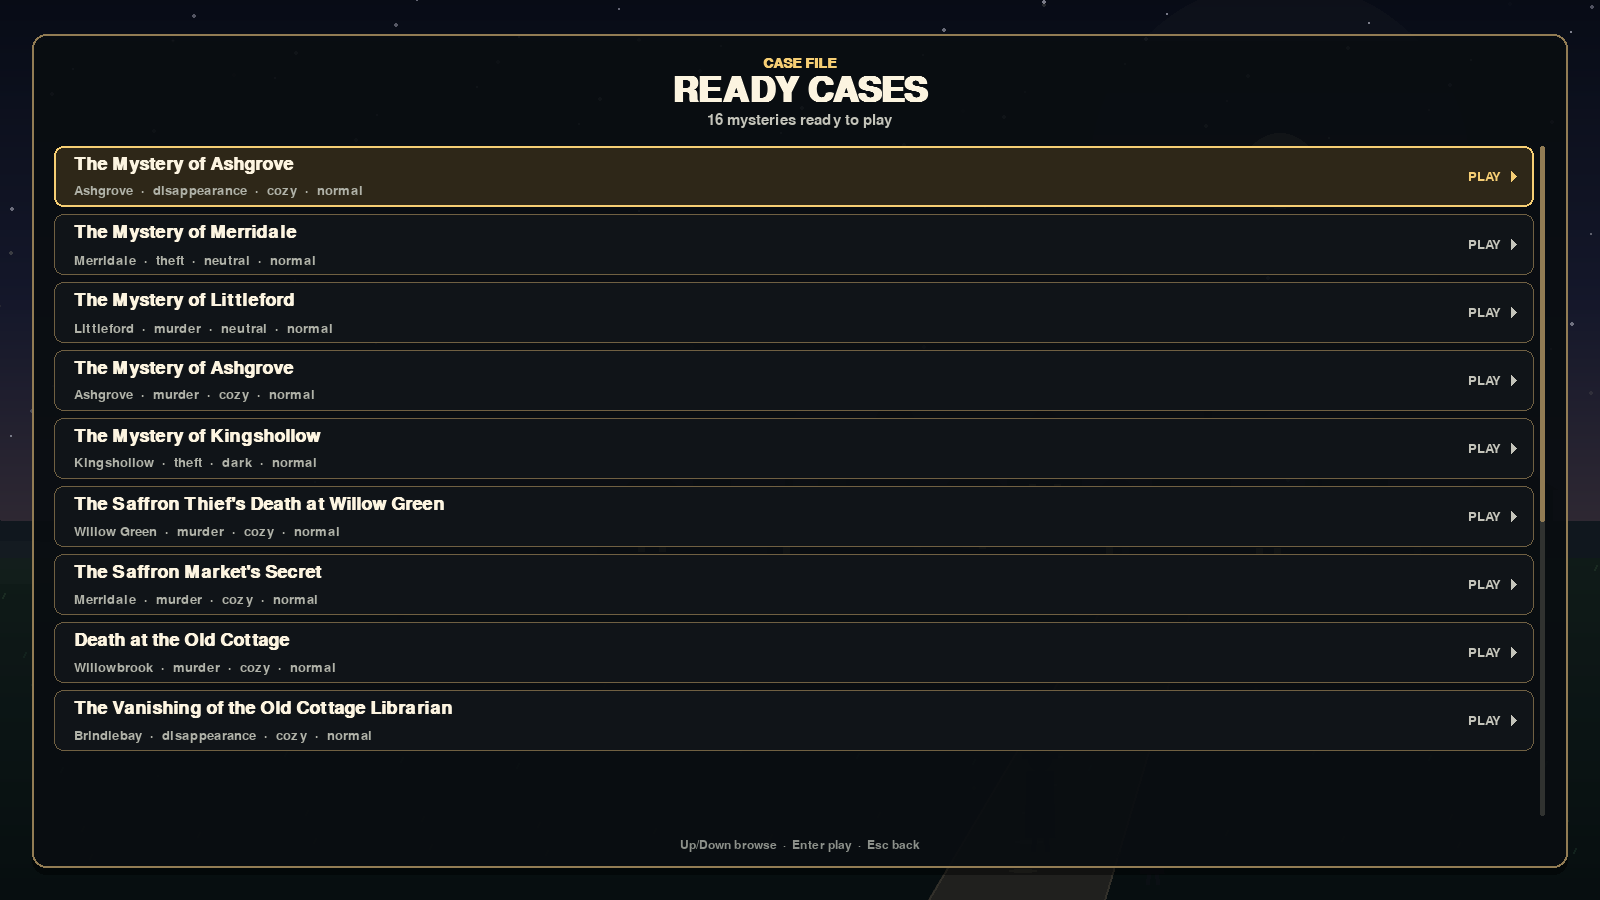
\includegraphics[width=\linewidth]{figures/case_picker.png}
    \caption{The curated case library. Sixteen validated bundles ship with the project.}
    \label{fig:cases}
  \end{subfigure}
  \caption{Case resolution and selection.}
  \label{fig:resolve}
\end{figure}

\begin{figure}[htbp]
  \centering
  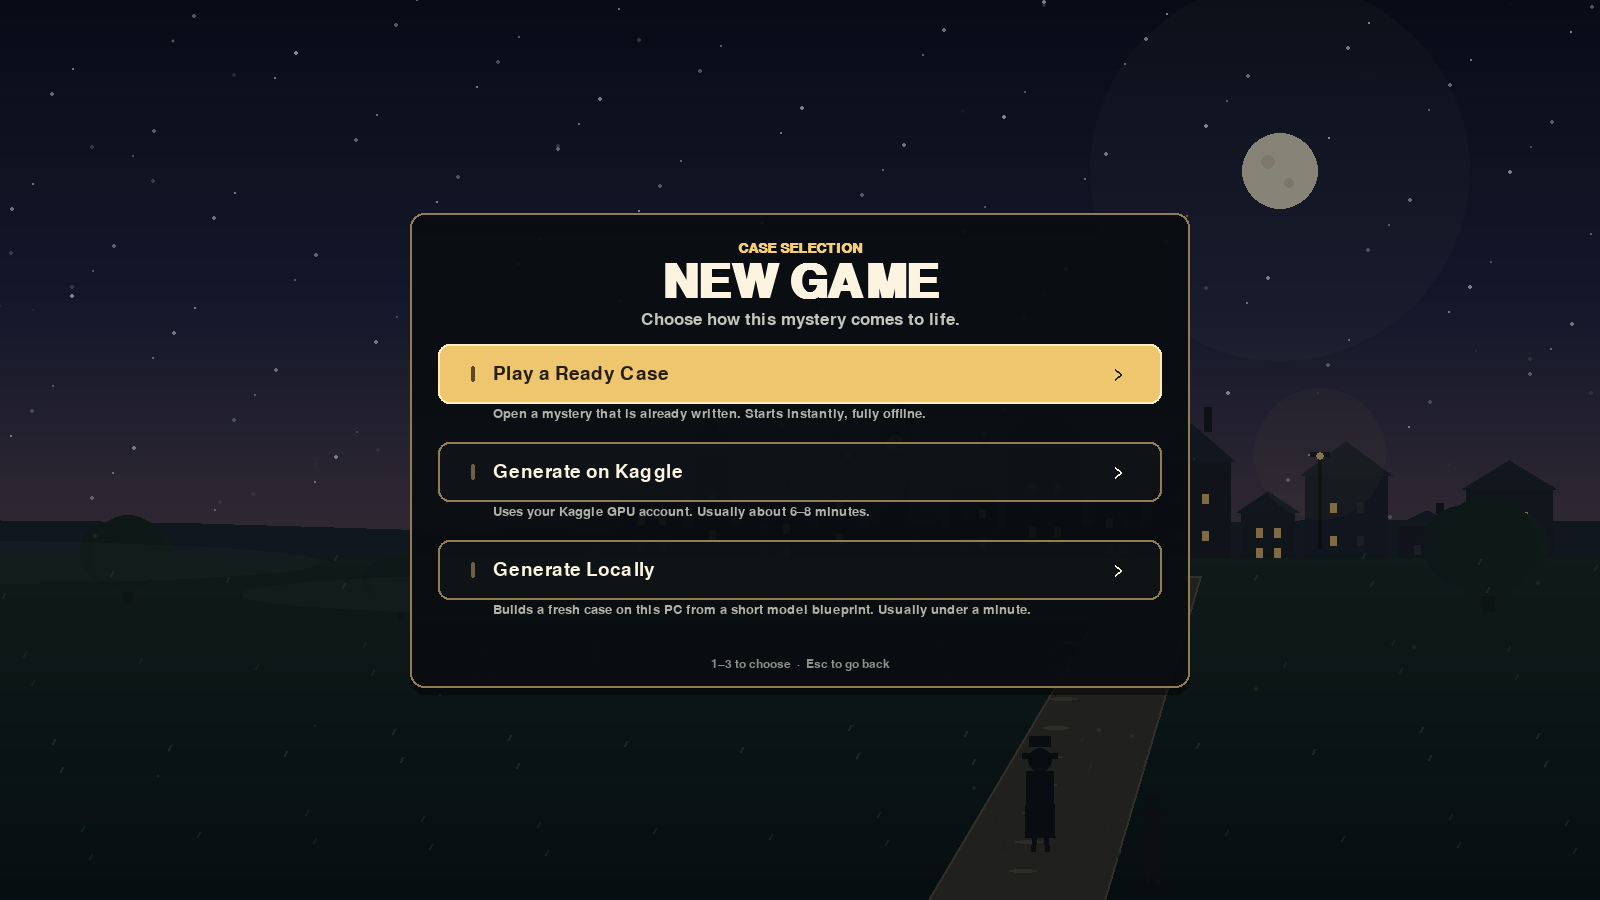
\includegraphics[width=0.68\textwidth]{figures/new_game.png}
  \caption{New game routes. ``Play a Ready Case'' starts instantly and offline; ``Generate on Kaggle'' and ``Generate Locally'' create a new bundle before play.}
  \label{fig:newgame}
\end{figure}

\section{Case Library and Offline Play}
Sixteen validated cases are curated in the repository. They cover all three mystery types, three tones, and both easy and normal difficulty, and they are regenerated only when the schema or compiler changes. The library is the offline showcase: a player can install the game, choose a ready case, and play without a model file, an API key, or a network connection. Local generation is an option, not a prerequisite.

\chapter{Evaluation}
\label{ch:eval}

\section{Research Questions and Protocol}
The evaluation asks four questions. \textbf{RQ1:} Does each route produce schema-valid bundles? \textbf{RQ2:} Are the bundles solvable, and is the proof recorded? \textbf{RQ3:} What are the end-to-end latency and memory costs on consumer hardware? \textbf{RQ4:} What does a small qualitative rubric reveal about narrative quality?

Runs were recorded against commit \texttt{852e10}, on an Intel Alder Lake-class CPU (Family 6, Model 154, Stepping 4) with 10 physical and 12 logical cores and 31.69\,GB of RAM, using 11 threads and temperature 0.6. Both model hashes matched the manifest. The protocol included five cold fast runs, thirty warm fast runs plus a discarded warm-up, nine fast repeats across three seeds, three staged runs (two valid, one failure), and one staged repeat. In total, 44 fast runs were included in the validity and latency statistics.

\begin{table}[htbp]
  \centering
  \small
  \begin{tabular}{@{}lrrrr@{}}
    \toprule
    \textbf{Route / condition} & \textbf{Records} & \textbf{Valid} & \textbf{Mean e2e (s)} & \textbf{Peak RSS (MB)} \\
    \midrule
    Fast 1B, cold & 5 & 5 & 9.803 & 1472.1 \\
    Fast 1B, warm & 30 & 30 & 9.032 & 1482.1 \\
    Fast 1B, repeats (3 seeds) & 9 & 9 & 8.976 & 1478.7 \\
    Staged 3B, cold & 3 & 2 & 657.662 & 3545.9 \\
    Staged 3B, repeat & 1 & 1 & 1363.304 & 3547.0 \\
    \bottomrule
  \end{tabular}
  \caption{Measurement matrix. The staged repeat is a case study, not an estimate; its extra model calls reflect retries. Warm-up records are excluded from the summary statistics.}
  \label{tab:runs}
\end{table}

\section{Validity and Solvability}
On the fast route, all 44 included runs produced a substantive blueprint (header, premise, cast, crime, at least one timeline entry, and at least one clue), parsed into the schema, passed the validator with zero issues, reached the culprit's deed through the clue chain, and passed the compiler's solvability proof. That is \good{44/44} on every gate. No run required a fallback to the synthetic blueprint library.

The staged route succeeded twice and failed once. The failure occurred after 628 seconds of inference and produced a bundle that did not pass final validation; it was not published. The two successful runs were valid and solvable. This is a small sample, but the direction is consistent with the architecture: longer free-form generation means more opportunities for a cross-stage inconsistency, and the final validator catches it only after the cost has been paid.

\section{Latency and Memory}
Warm fast generation averaged 9.03 seconds end-to-end (median 9.01, SD 0.60), including 9.01 seconds of model inference and 25 milliseconds of parsing, validation, compilation, and publication. Output averaged 279 tokens at 31.0 tokens/s. Cold runs added about one second of model load. Peak RSS was 1.48\,GB.

Staged generation averaged 657.7 seconds for the two valid cold runs (623.2 and 692.2), at 5.27 tokens/s and 3.55\,GB peak RSS. The single repeat with retries took 1,363 seconds at 2.69 tokens/s. The end-to-end speed-up of the fast route is $657.662/9.032=72.8\times$; the memory ratio is $3545.9/1482.1=2.39\times$.

\begin{figure}[htbp]
  \centering
  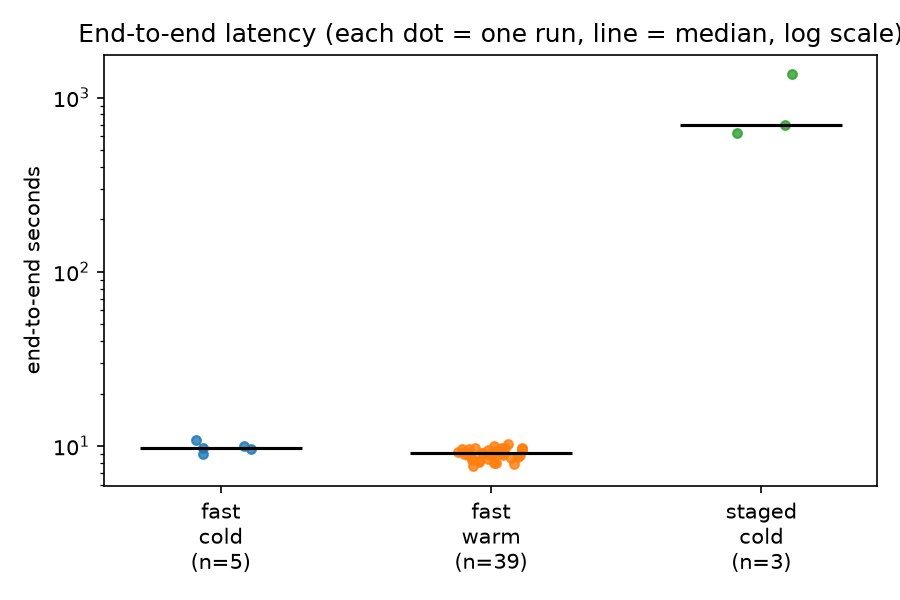
\includegraphics[width=0.82\textwidth]{figures/latency_groups.png}
  \caption{End-to-end latency by condition (log scale). Each dot is one run; the horizontal line is the median. Fast runs cluster around nine seconds; staged runs are two orders of magnitude slower.}
  \label{fig:latency-groups}
\end{figure}

\begin{figure}[htbp]
  \centering
  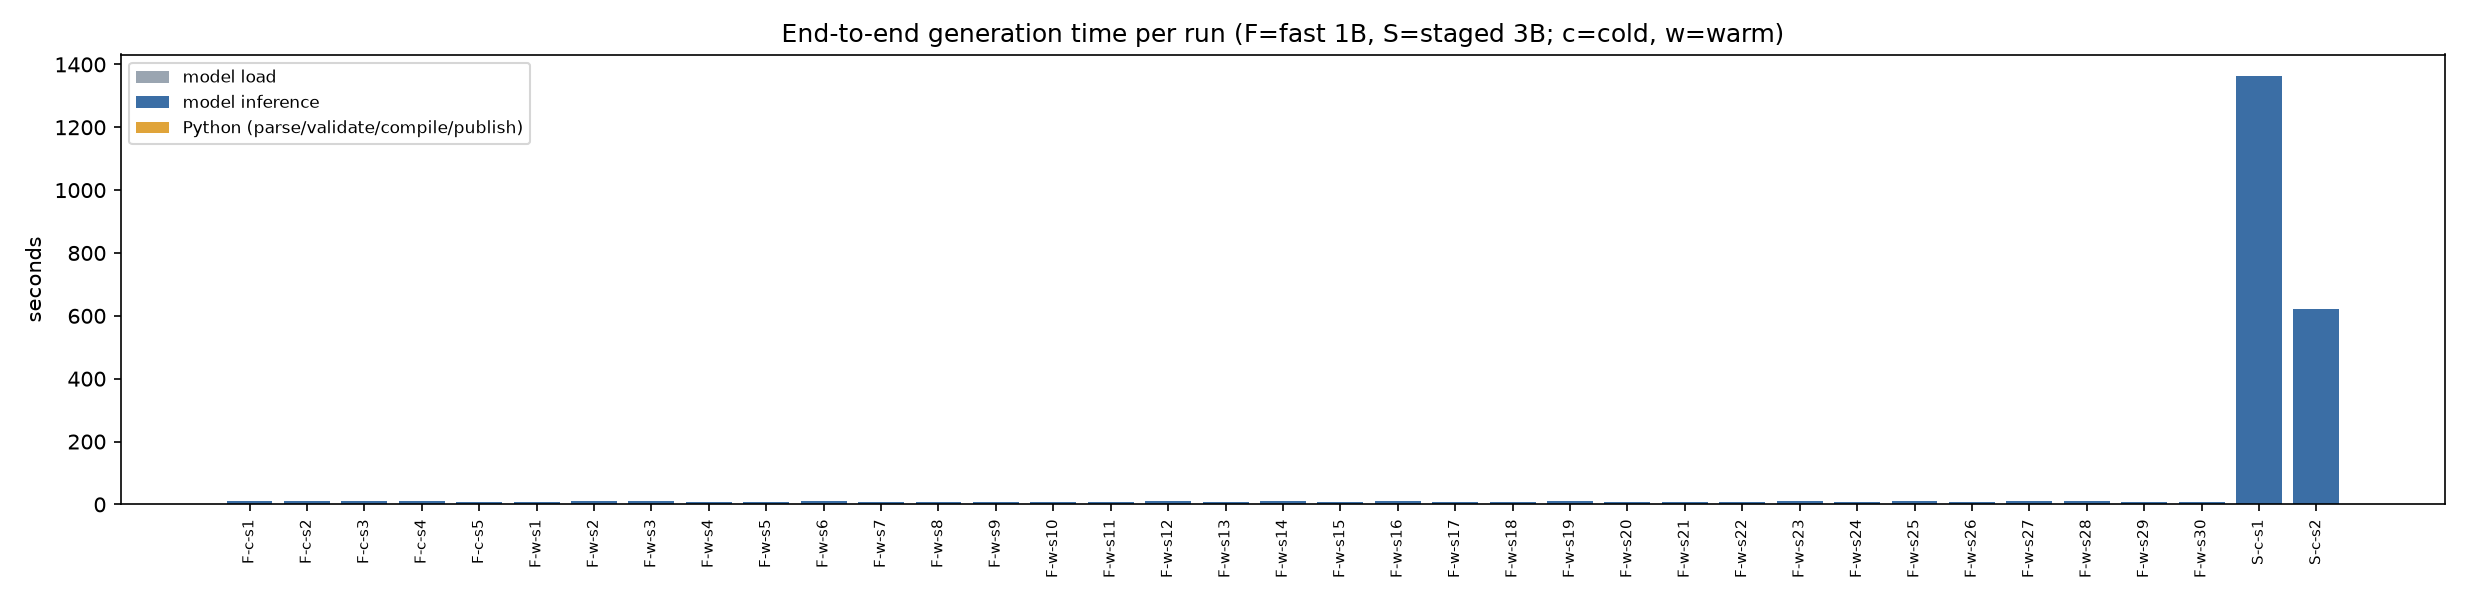
\includegraphics[width=\textwidth]{figures/latency_breakdown.png}
  \caption{Per-run breakdown. Model load is a small fraction of cold fast runs; on staged runs, inference dominates completely.}
  \label{fig:latency-breakdown}
\end{figure}

\begin{figure}[htbp]
  \centering
  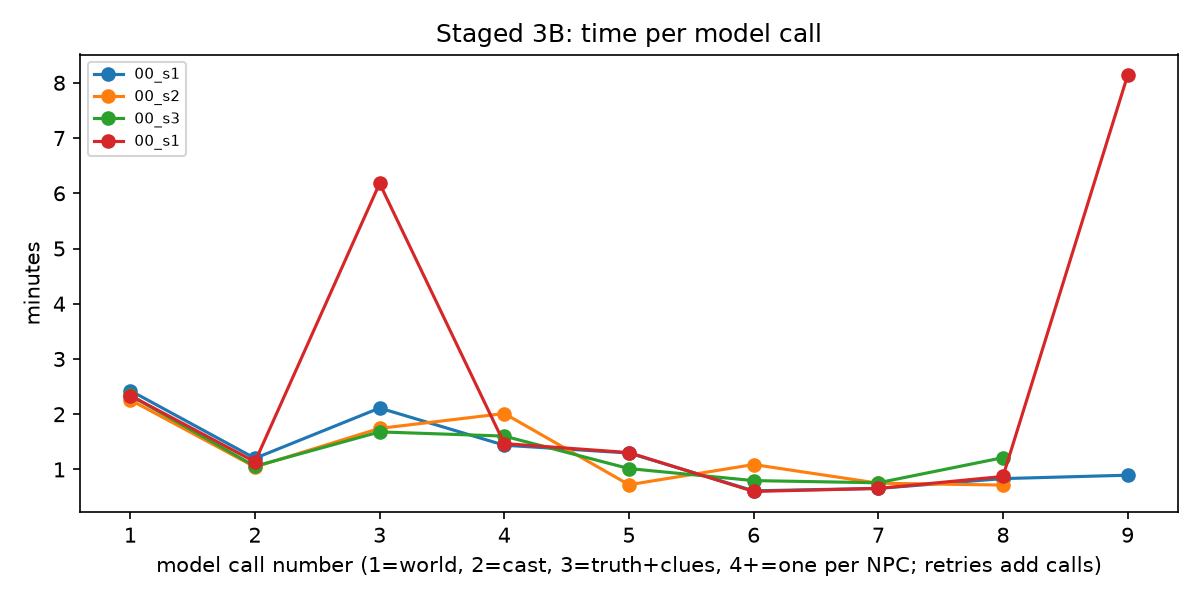
\includegraphics[width=0.8\textwidth]{figures/staged_calls.png}
  \caption{Staged route cost per model call. The first three calls build the world, cast, and truth/clues; later calls produce each NPC. Retries add calls and can dominate the total.}
  \label{fig:staged-calls}
\end{figure}

\section{Narrative Quality}
Four generated cases were scored by a human rater on six dimensions, each from 1 to 5. The rubric covers logical consistency, mystery coherence, clue relevance, NPC identity/memory consistency, human solvability, and narrative quality. The sample is deliberately small; it is a diagnostic, not a benchmark.

\begin{table}[htbp]
  \centering
  \footnotesize
  \setlength{\tabcolsep}{3.5pt}
  \begin{tabular}{@{}lccccccl@{}}
    \toprule
    \textbf{Case} & \textbf{Logic} & \textbf{Coherence} & \textbf{Clues} & \textbf{Memory} & \textbf{Solvable} & \textbf{Prose} & \textbf{Notes} \\
    \midrule
    case\_124 & 2 & 5 & 3 & 5 & 4 & 2 & broken English, internal ids \\
    case\_249 & 2 & 4 & 2 & 2 & 2 & 2 & location contradiction \\
    case\_339 & 2 & 5 & 3 & 5 & 5 & 4 & item mismatch in title \\
    case\_979 & 3 & 3 & 1 & 4 & 1 & 3 & clues name no one \\
    \midrule
    \textbf{Mean} & \textbf{2.25} & \textbf{4.25} & \textbf{2.25} & \textbf{4.00} & \textbf{3.00} & \textbf{2.75} & \\
    \bottomrule
  \end{tabular}
  \caption{Qualitative rubric scores (1--5). Mystery coherence and per-NPC memory consistency are strong; clue specificity and surface prose are the weak points. Two entries in the raw sheet carry rater notes and should be treated as provisional.}
  \label{tab:rubric}
\end{table}

The pattern is informative. The architecture does what it was designed to do: characters stay coherent, memories do not leak, and the solution is usually reachable. The failures are about \emph{surface specificity}. Clues such as ``a physical trace: theft trace'' are formally linked to a culprit fact but give the player nothing to reason with. Internal identifiers (\texttt{loc\_library}, \texttt{npc\_baker}) occasionally leak into player-facing text. Titles and intros can disagree about the stolen item. These are not architectural failures; they are prompt, schema, and post-processing gaps, and they define the next iteration.

\section{Reproducibility and Diversity}
Across 31 distinct seeds the fast route produced 31 distinct bundles, five distinct titles, and fifteen distinct culprit names. Same-seed repeats were mostly stable but not perfectly so: two of five seeds produced two distinct bundles across repetitions, which is expected at temperature 0.6. The practical consequence is that a case is reproducible when its seed, model hash, and settings are recorded, but not bit-identical across every rerun. The evaluation records all three.

\section{Threats to Validity}
The staged sample is small (two valid runs), so its mean is a case study rather than an estimate. All measurements come from one machine; the 72.8-fold gap is robust to reasonable hardware variation because it is driven by token count and model size, but the absolute latencies are not portable. The rubric has four cases and two provisional entries, and it was scored by one rater. Live-provider behaviour was not part of this run: keys, judge protocol, and the probe suite belong to the next evaluation phase, and the scripted fallback is excluded from provider metrics by design.

\chapter{Discussion}
\label{ch:discussion}

\section{What the Speed-Up Actually Measures}
The 72.8-fold gap is not a tuning trick. It decomposes into roughly twelve times fewer output tokens and roughly six times higher token throughput, and the product is the measured ratio. Fewer tokens come from replacing JSON with a dense DSL; higher throughput comes from using a 1B model instead of a 3B model and from avoiding a grammar mask over a 152k-token vocabulary on every step. Neither factor depends on a GPU. Both are consequences of the division of labour.

\section{Fidelity Versus Reliability}
A compiler that fills structural gaps can make a weak sketch playable, but it cannot make it interesting. This is the central trade-off of the project. The blueprint route achieves near-perfect structural validity and solvability, yet its clue prose is often generic, and the compiled world sometimes reads as a template. The staged route is more expressive in principle, but its global consistency is fragile and its latency is two orders of magnitude worse. The right next step is not to abandon the compiler but to give the sketch a richer vocabulary for the parts that matter to the player: clue text, location description, and the culprit's cover story.

\section{Isolation as an Architectural Property}
The spoiler firewall is often described as a prompting concern. In Fabula it is a data-flow property. The conversation service receives a directory of per-NPC files, not the bundle root. The truth file is not in that directory. The prompt assembler therefore cannot include it, and tests assert that canary strings never cross the boundary. This is a stronger guarantee than instruction-following, and it is the main reason the memory-consistency rubric scores are high even when prose quality is uneven.

\section{Limitations}
\begin{itemize}
  \item \textbf{Clue specificity.} Formally linked clues can still be narratively empty. The rubric's clue-relevance mean of 2.25 is the clearest failure.
  \item \textbf{Surface text.} Internal identifiers and broken phrasing occasionally reach the player. A post-processing pass and a stricter schema for player-facing strings would help.
  \item \textbf{Small qualitative sample.} Four cases and one rater cannot support a claim about average narrative quality.
  \item \textbf{Live conversation untested here.} Provider robustness, latency, and disclosure adherence require the probe suite and API keys; this report measures generation, not live dialogue.
  \item \textbf{Staged route viability.} The 3B staged route is too slow for the product. It survives as a comparison and as a teacher, not as a shipping path.
\end{itemize}

\section{Future Work}
\begin{enumerate}
  \item \textbf{Richer DSL fields.} Add optional prose slots for clue text, location description, and cover story, and train the student to use them without inflating the token budget.
  \item \textbf{Post-processing and linting.} Replace internal identifiers with display names, reject title/item mismatches, and enforce a minimum specificity for clue descriptions.
  \item \textbf{Probe-based NPC evaluation.} Run the planned secret-keeping, false-confession, persona, and disclosure probes against at least two live providers, with the scripted baseline reported separately.
  \item \textbf{A larger human study.} Score more cases with multiple raters and report agreement, so that narrative quality can be compared across routes rather than only described.
  \item \textbf{Smaller or faster students.} Evaluate a 1.5B student and a grammar-light JSON variant to see whether the compiler advantage survives with more expressive output.
\end{enumerate}

\chapter{Conclusion}
\label{ch:conclusion}

Fabula began with a simple observation: a ten-minute mystery game cannot spend half an hour generating its case, and a small language model cannot reliably maintain a game world as JSON. The project's answer is a neurosymbolic division of labour. A fine-tuned 1B model writes a compact blueprint---premise, cast, crime, timeline, clues---and a deterministic compiler expands it into a validated, provably solvable bundle. The play phase is classical and headless; the language model returns only as an optional voice, bounded by per-NPC knowledge and a spoiler firewall.

The evaluation supports the design. The fast route was valid and solvable in 44 out of 44 measured runs, averaged 9.03 seconds warm on a laptop CPU, used 1.48\,GB of memory, and was 72.8 times faster end-to-end than the staged 3B route. A small rubric shows strong coherence and memory isolation, and pinpoints clue specificity and prose as the remaining quality gaps.

The broader lesson is that generative game content benefits from an explicit boundary between \emph{what the model imagines} and \emph{what the engine can prove}. The boundary makes cases fast, testable, and safe to publish. It also makes the next iteration tractable: improve the sketch, and the compiler will carry it.

% ===========================================================================
% REFERENCES
% ===========================================================================
\clearpage
\phantomsection
\addcontentsline{toc}{chapter}{References}
\begin{thebibliography}{99}
\small

\bibitem{park2023generative}
J.~S. Park, J.~C. O'Brien, C.~J. Cai, M.~R. Morris, P.~Liang, and M.~S. Bernstein.
\newblock Generative agents: Interactive simulacra of human behavior.
\newblock In \emph{Proceedings of the 36th Annual ACM Symposium on User Interface Software and Technology (UIST)}, 2023.

\bibitem{yao2023react}
S.~Yao, J.~Zhao, D.~Yu, N.~Du, I.~Shafran, K.~Narasimhan, and Y.~Cao.
\newblock ReAct: Synergizing reasoning and acting in language models.
\newblock In \emph{International Conference on Learning Representations (ICLR)}, 2023.

\bibitem{wang2023voyager}
G.~Wang, Y.~Xie, Y.~Jiang, A.~Mandlekar, C.~Xiao, Y.~Zhu, L.~Fan, and A.~Anandkumar.
\newblock Voyager: An open-ended embodied agent with large language models.
\newblock \emph{Transactions on Machine Learning Research}, 2024. arXiv:2305.16291.

\bibitem{ammanabrolu2020quest}
P.~Ammanabrolu and M.~O. Riedl.
\newblock Toward automated quest generation in text-adventure games.
\newblock In \emph{Proceedings of the 16th Conference on Computational Intelligence and Games (CIG)}, 2020.

\bibitem{garcez2023neurosymbolic}
A.~d'Avila Garcez and L.~C. Lamb.
\newblock Neurosymbolic AI: The 3rd wave.
\newblock \emph{Artificial Intelligence Review}, 56:12387--12406, 2023.

\bibitem{kautz2022third}
H.~Kautz.
\newblock The third AI summer.
\newblock \emph{Proceedings of the AAAI Conference on Artificial Intelligence}, 36(9):12312--12320, 2022.

\bibitem{willard2023guided}
B.~T. Willard and R.~Louf.
\newblock Efficient guided generation for large language models.
\newblock arXiv:2307.09702, 2023.

\bibitem{knox1929decalogue}
R.~A. Knox.
\newblock A detective story decalogue.
\newblock In \emph{The Bookman Anthology}, 1929.

\bibitem{vandine1928rules}
S.~S. Van~Dine.
\newblock Twenty rules for writing detective stories.
\newblock \emph{The American Magazine}, 1928.

\bibitem{hu2022lora}
E.~J. Hu, Y.~Shen, P.~Wallis, Z.~Allen-Zhu, Y.~Li, S.~Wang, L.~Wang, and W.~Chen.
\newblock LoRA: Low-rank adaptation of large language models.
\newblock In \emph{International Conference on Learning Representations (ICLR)}, 2022.

\bibitem{dettmers2023qlora}
T.~Dettmers, A.~Pagnoni, A.~Holtzman, and L.~Zettlemoyer.
\newblock QLoRA: Efficient finetuning of quantized LLMs.
\newblock In \emph{Advances in Neural Information Processing Systems (NeurIPS)}, 2023.

\bibitem{llama3herd}
Llama Team, AI@Meta.
\newblock The Llama 3 herd of models.
\newblock arXiv:2407.21783, 2024.

\bibitem{qwen2025}
Qwen Team.
\newblock Qwen2.5 technical report.
\newblock arXiv:2412.15115, 2024.

\bibitem{unsloth}
Unsloth AI.
\newblock Unsloth: Fast, memory-efficient fine-tuning of large language models.
\newblock Software documentation, 2024--2026. \url{https://github.com/unslothai/unsloth}.

\bibitem{llamacpp}
G.~Gerganov et al.
\newblock \texttt{llama.cpp}: LLM inference in C/C++.
\newblock Software, 2023--2026. \url{https://github.com/ggml-org/llama.cpp}.

\bibitem{pydantic}
Pydantic Services Inc.
\newblock Pydantic: Data validation using Python type hints.
\newblock Software documentation. \url{https://docs.pydantic.dev}.

\bibitem{pygame}
Pygame Community.
\newblock Pygame: Python game development library.
\newblock Software documentation. \url{https://www.pygame.org}.

\end{thebibliography}

% ===========================================================================
% APPENDICES
% ===========================================================================
\appendix
\chapter{Bundle Excerpt}
\label{app:bundle}

The following excerpt shows the shape of a published bundle. It is taken from the sample case distributed with the project and abbreviated for readability.

\begin{lstlisting}[style=bundle]
{
  "schema_version": "1.0",
  "scenario_id": "theft_3",
  "mystery_type": "theft",
  "tone": "cozy",
  "difficulty": "easy",
  "title": "The Stolen silver locket",
  "town_name": "Brindlebay",
  "locations": [
    {"id": "loc_residence", "name": "Lane House", "type": "residence",
     "connections": ["loc_library"], "clue_spots": ["clue_02"]},
    {"id": "loc_library", "name": "Old Library", "type": "library",
     "connections": ["loc_residence", "loc_market"], "clue_spots": ["clue_01"]}
  ],
  "npcs": [
    {"id": "npc_01", "display_name": "Ivy", "start_location": "loc_park",
     "schedule": [{"at_minute": 1, "location": "loc_park"},
                  {"at_minute": 5, "location": "loc_residence"}]}
  ]
}
\end{lstlisting}

A memory file contains facts rather than prose:

\begin{lstlisting}[style=bundle]
{
  "npc_id": "npc_02",
  "facts": [
    {"who": "npc_02", "kind": "observation", "source": "did",
     "secret": false, "disclosure": "volunteer",
     "content": "I locked the reading room at closing time."},
    {"who": "npc_02", "kind": "alibi", "source": "did",
     "secret": false, "disclosure": "volunteer",
     "content": "I was at the park at minute seven."}
  ]
}
\end{lstlisting}

The truth file is never part of a prompt. It is used by the accusation service and by the validators:

\begin{lstlisting}[style=bundle]
{
  "solution": {
    "correct_culprit_id": "npc_02",
    "correct_method_id": "m_method_1",
    "correct_motive_id": "m_motive_1"
  },
  "crime": {"scene": "loc_library", "minute": 5}
}
\end{lstlisting}

\chapter{Reproducibility Commands}
\label{app:repro}

The project is a Python package with a CLI. The following commands reproduce the main artefacts. Model weights are not committed; the manifest records the expected hashes.

\begin{lstlisting}[style=bundle]
# Install and verify the model artifact
python -m pip install -e .
python -m pip install llama-cpp-python --prefer-binary \
  --extra-index-url https://abetlen.github.io/llama-cpp-python/whl/cpu
python -m fabula model check

# Generate a case with the fast blueprint route
python -m fabula generate --fast --type theft --seed 1 --out bundles/my-case

# Play a ready case / launch the client
python -m fabula play bundle
python -m fabula

# Quality gates
python -m pytest
python -m ruff check .
python -m ruff format --check .
\end{lstlisting}

Training programs live in \texttt{training/scripts/} and are designed for Kaggle notebooks. The teacher expansion, staged 3B SFT, DSL distillation, and 1B student SFT are separate scripts so that each stage can be re-run without repeating the others. Evaluation records, model manifests, and the rubric sheet are committed; raw model outputs and weights are not.

\vspace{0.6cm}
\begin{keybox}[One-line reproduction]
\begin{center}
\texttt{python -m fabula generate --fast --type theft --seed 1}
\end{center}
A warm CPU run produces a validated, solvability-proved case in about nine seconds. The same seed and model hash reproduce the same request; the case itself may vary slightly at temperature 0.6.
\end{keybox}

\end{document}
